\documentclass%
%[handout]
{beamer}
% % % % % % % %
% % % % % % % %
% % % % % % % %
%IMPORTANT
%compiles with 
%pdflatex -shell-escape 
%IMPORTANT
% % % % % % % %
% % % % % % % %
% % % % % % % %
\mode<presentation>
{
\useinnertheme{rounded}
\useoutertheme{infolines}
\usecolortheme{orchid}
\usecolortheme{whale}
}

\usepackage[english]{babel}
\usepackage[latin1]{inputenc}
\usepackage[all,cmtip]{xy}
\usepackage{times}
\usepackage[T1]{fontenc}
\usepackage{../example-templates}
\usepackage{../pstricks-commands}

\usepackage{auto-pst-pdf}
\usepackage{pst-plot}
%\usepackage{pstricks-add} 

% Or whatever. Note that the encoding and the font should match. If T1
% does not look nice, try deleting the line with the fontenc.


\graphicspath{{../../modules/}}

\newtheoremstyle{partialproof}{3pt}{3pt}{}{}{}{.}{.5em}{}
\theoremstyle{partialproof} \newtheorem{partialproof}[theorem]{Proof.}
%\DeclareMathOperator{\diff}{d}
\setbeamertemplate{navigation symbols}{}

\includeonlylecture{1}

\newcommand{\lect}[3]{
  \date{#1}
  \lecture[#1]{#2}{#3}
}

\setbeamertemplate{footline}
{
  \leavevmode%
  \hbox{%
  \begin{beamercolorbox}[wd=.333333\paperwidth,ht=2.25ex,dp=1ex,center]{author in head/foot}%
    \usebeamerfont{author in head/foot}\insertshortauthor
  \end{beamercolorbox}%
  \begin{beamercolorbox}[wd=.333333\paperwidth,ht=2.25ex,dp=1ex,center]{title in head/foot}%
    \usebeamerfont{title in head/foot}\insertshorttitle
  \end{beamercolorbox}%
  \begin{beamercolorbox}[wd=.333333\paperwidth,ht=2.25ex,dp=1ex,center]{date in head/foot}%
    \usebeamerfont{date in head/foot}\insertshortdate{}
  \end{beamercolorbox}}%
  \vskip0pt%
}

% If you have a file called "university-logo-filename.xxx", where xxx
% is a graphic format that can be processed by latex or pdflatex,
% resp., then you can add a logo as follows:

%\pgfdeclareimage[height=0.8cm]{logo}{bluelogo}
%\logo{\pgfuseimage{logo}}
\renewcommand{\Arcsin}{\arcsin}
\renewcommand{\Arccos}{\arccos}
\renewcommand{\Arccot}{\text{arccot}}
\renewcommand{\Arctan}{\arctan}


\begin{document}

\AtBeginLecture{%

\title[\insertlecture]{FreeCalc}
\subtitle{\insertlecture}
\author[FreeCalc]{}
\institute[UMass Boston]{University of Massachusetts Boston}
\date{\insertshortlecture}
\begin{frame}
  \titlepage
\end{frame}
}%

% begin lecture
\lect{\today}{Sample}{1}

\begin{frame}
\frametitle{Geometric interpretation of all trigonometric functions}
\begin{columns}
\column{0.4\textwidth}
\psset{xunit=1.5cm,yunit=1.5cm}
\begin{pspicture}(0,-2)(5,3)
\tiny
\rput[rb](-0.1,1){$1$}
%circle:
\psplot[linecolor=\psColorGraph, plotpoints=1000]{-1.000000}{1.000000}{1 x 2 exp -1 mul add sqrt }
\psplot[linecolor=\psColorGraph, plotpoints=1000]{-1.000000}{1.000000}{1 x 2 exp -1 mul add sqrt -1 mul }
\psline(1, -2.5)(1,2.5)

\uncover<2->{
\psline(0,0)(1,2)
}
\psline[linecolor=green](0,0)(0.447213595,0)

%angle:
\psaxes[ticks=none, labels=none]{<->}(0,0)(-1.2,-1.2)(1.2,1.2)

\uncover<2->{
\rput[lb](0.3, 0.2){\alert<2>{$\theta$}}
\psplot[plotpoints=1000]{0.134164079}{0.2999}{0.09 x 2 exp -1 mul add sqrt}
\rput[l](1.05,2){\alert<2>{$B$}}
\rput[bl](1.05,0.05){\alert<2>{$D$}}
}

\psline(0.95,0)(0.95, 0.05)(1,0.05)

\rput[tr](-0.1,-0.1){\alert<2>{$O$}}
\uncover<3->{
\rput[b](0.4,1){\alert<3>{$A$}}
}


\uncover<5->{
\psline[linecolor=blue](0.447213595, 0.894427191)(0.447213595,0)
\rput[tl](0.45,-0.05){$C$}
\psline(0.397213595,0)(0.397213595, 0.05)(0.447213595,0.05)
}

\uncover<6->{
\psline[linecolor=green](0,0)(0.447213595,0)
}
\uncover<7->{
\psline[linecolor=purple](1,0)(1,2)
}
\uncover<8->{
\psline[linecolor=cyan](1,0)(1,-0.5)
\rput[l](1.05,-0.5){$E$}
\psline[linecolor=black](0,0)(1,-0.5)
\psline(0.04472136,-0.02236068)(0.06708204,0.02236068) (0.02236068, 0.04472136)
}
\uncover<9->{
\psline[linecolor=orange](0,0)(1,-0.5)
}
\uncover<10->{
\psline[linecolor=magenta](0,0)(1,2)
}
\end{pspicture}
\column{0.6\textwidth}
On picture: circle of radius $1$ centered at point $O$ with coordinates $(0,0)$. \uncover<2->{Let \alert<2>{$\angle DOB=\theta$}.} \uncover<3->{\alert<3>{Let $OB$ intersect the circle at point $A$}.} \uncover<4->{Then the coordinates of $A$ are $(\color{blue}\sin\theta \color{black},\color{green}\cos \theta\color{black} )$.}

\medskip

\uncover<5->{ $\color{blue}\sin \theta \color{black} = \frac{|AC|}{|OA|} = \frac{|AC|}{1}=|AC| $.}

\uncover<6->{ $\color{green}\cos \theta \color{black} =\frac{|OC|}{|OA|}=\frac{|OC|}{1}= |OC| $.}

\uncover<7->{$\color{purple} \tan \theta\color{black} = \frac{|BD|}{|OD|}=\frac{|BD|}{1}=|BD|$.}

\uncover<8->{$\color{cyan} \cot \theta\color{black} = \frac{|DE|}{|OD|}=\frac{|DE|}{1}=|DE|$.} 


\uncover<9->{$ \color{orange}\csc\theta \color{black} =\frac{|OE|}{|DO|}=\frac{|OE|}{1}=|OE|$.}

\uncover<10->{$\color{magenta} \sec\theta \color{black} =\frac{|OB|}{|OD|}=\frac{|OB|}{1}=|OB|$.}

\end{columns}
\end{frame}
% begin module areas-intro


\begin{frame}
\frametitle{The Area Problem}
\begin{itemize}
\item  How can we find the area under $y = x^2$ between $x = 0$ and $x = 1$?
\item<handout:2-| 2->  We can approximate it using rectangles.
\item<handout:2-| 3->  Divide $[0,1]$ into three strips of width $\frac{1}{3}$, and draw rectangles in those strips, the heights of which are the same as the height of the function at the right end of that strip.
\item<handout:3-| 4->  Four strips gives a better approximation. \uncover<handout:0| 5->{Five is even better.}
\item<handout:6-| 11-19>  We could use the left endpoints to find the heights instead.
\end{itemize}
\begin{center}
\psset{xunit=2cm, yunit=2cm}
\begin{pspicture}(-0.15,-0.15)(1.45,1.45)
\psline{linecolor=red!1}(0, -0.3)(0, -0.31)
\psframe*[linecolor=white](-0.15,-0.15)(1.45,1.45)
\tiny
\psline(-0.05, 1)(0.05,1)
\rput[r] (-0.07,1){$1$}
%Function formula: x^{2}
\rput(0.9,1.3){$y=x^{2}$}
\uncover<handout:2|3,12>{
%approximation 1/3
\psline*[linecolor=\fcColorAreaUnderGraph, linewidth=0.1pt](0.333333, 0)(0.333333, 0.111111)(0, 0.111111)(0, 0)(0.666667, 0)(0.666667, 0.444444)(0.333333, 0.444444)(0.333333, 0)(1, 0)(1, 1)(0.666667, 1)(0.666667, 0)
\psline[linecolor=blue, linewidth=0.1pt](0.333333, 0)(0.333333, 0.111111)(0, 0.111111)(0, 0)(0.666667, 0)(0.666667, 0.444444)(0.333333, 0.444444)(0.333333, 0)(1, 0)(1, 1)(0.666667, 1)(0.666667, 0)
\rput[t](0.333333,-0.03){$\frac{1}{3}$}\rput[t](0.666667,-0.03){$\frac{2}{3}$}\rput[t](1,-0.03){$1$}
}
\uncover<handout:3,6|4,13>{
%approximation 1/4
\psline*[linecolor=\fcColorAreaUnderGraph, linewidth=0.1pt](0.25, 0)(0.25, 0.0625)(0, 0.0625)(0, 0)(0.5, 0)(0.5, 0.25)(0.25, 0.25)(0.25, 0)(0.75, 0)(0.75, 0.5625)(0.5, 0.5625)(0.5, 0)(1, 0)(1, 1)(0.75, 1)(0.75, 0)
\psline[linecolor=blue, linewidth=0.1pt](0.25, 0)(0.25, 0.0625)(0, 0.0625)(0, 0)(0.5, 0)(0.5, 0.25)(0.25, 0.25)(0.25, 0)(0.75, 0)(0.75, 0.5625)(0.5, 0.5625)(0.5, 0)(1, 0)(1, 1)(0.75, 1)(0.75, 0)
\rput[t](0.25,-0.03){$\frac{1}{4}$}\rput[t](0.5,-0.03){$\frac{1}{2}$}\rput[t](0.75,-0.03){$\frac{3}{4}$}\rput[t](1,-0.03){$1$}
}
\uncover<handout:0|5,14>{
%approximation 1/5
\psline*[linecolor=\fcColorAreaUnderGraph, linewidth=0.1pt](0.2, 0)(0.2, 0.04)(0, 0.04)(0, 0)(0.4, 0)(0.4, 0.16)(0.2, 0.16)(0.2, 0)(0.6, 0)(0.6, 0.36)(0.4, 0.36)(0.4, 0)(0.8, 0)(0.8, 0.64)(0.6, 0.64)(0.6, 0)(1, 0)(1, 1)(0.8, 1)(0.8, 0)
\psline[linecolor=blue, linewidth=0.1pt](0.2, 0)(0.2, 0.04)(0, 0.04)(0, 0)(0.4, 0)(0.4, 0.16)(0.2, 0.16)(0.2, 0)(0.6, 0)(0.6, 0.36)(0.4, 0.36)(0.4, 0)(0.8, 0)(0.8, 0.64)(0.6, 0.64)(0.6, 0)(1, 0)(1, 1)(0.8, 1)(0.8, 0)
\rput[t](0.2,-0.03){$\frac{1}{5}$}\rput[t](0.4,-0.03){$\frac{2}{5}$}\rput[t](0.6,-0.03){$\frac{3}{5}$}\rput[t](0.8,-0.03){$\frac{4}{5}$}\rput[t](1,-0.03){$1$}
}
\uncover<handout:0|6,15>{
%approximation 1/8
\psline*[linecolor=\fcColorAreaUnderGraph, linewidth=0.1pt](0.125, 0)(0.125, 0.015625)(0, 0.015625)(0, 0)(0.25, 0)(0.25, 0.0625)(0.125, 0.0625)(0.125, 0)(0.375, 0)(0.375, 0.140625)(0.25, 0.140625)(0.25, 0)(0.5, 0)(0.5, 0.25)(0.375, 0.25)(0.375, 0)(0.625, 0)(0.625, 0.390625)(0.5, 0.390625)(0.5, 0)(0.75, 0)(0.75, 0.5625)(0.625, 0.5625)(0.625, 0)(0.875, 0)(0.875, 0.765625)(0.75, 0.765625)(0.75, 0)(1, 0)(1, 1)(0.875, 1)(0.875, 0)
\psline[linecolor=blue, linewidth=0.1pt](0.125, 0)(0.125, 0.015625)(0, 0.015625)(0, 0)(0.25, 0)(0.25, 0.0625)(0.125, 0.0625)(0.125, 0)(0.375, 0)(0.375, 0.140625)(0.25, 0.140625)(0.25, 0)(0.5, 0)(0.5, 0.25)(0.375, 0.25)(0.375, 0)(0.625, 0)(0.625, 0.390625)(0.5, 0.390625)(0.5, 0)(0.75, 0)(0.75, 0.5625)(0.625, 0.5625)(0.625, 0)(0.875, 0)(0.875, 0.765625)(0.75, 0.765625)(0.75, 0)(1, 0)(1, 1)(0.875, 1)(0.875, 0)
\rput[t](0.125,-0.03){$\frac{1}{8}$}\rput[t](0.25,-0.03){$\frac{1}{4}$}\rput[t](0.375,-0.03){$\frac{3}{8}$}\rput[t](0.5,-0.03){$\frac{1}{2}$}\rput[t](0.625,-0.03){$\frac{5}{8}$}\rput[t](0.75,-0.03){$\frac{3}{4}$}\rput[t](0.875,-0.03){$\frac{7}{8}$}\rput[t](1,-0.03){$1$}
}
\uncover<handout:4|7,16>{
%approximation 1/10
\psline*[linecolor=\fcColorAreaUnderGraph, linewidth=0.1pt](0.1, 0)(0.1, 0.01)(0, 0.01)(0, 0)(0.2, 0)(0.2, 0.04)(0.1, 0.04)(0.1, 0)(0.3, 0)(0.3, 0.09)(0.2, 0.09)(0.2, 0)(0.4, 0)(0.4, 0.16)(0.3, 0.16)(0.3, 0)(0.5, 0)(0.5, 0.25)(0.4, 0.25)(0.4, 0)(0.6, 0)(0.6, 0.36)(0.5, 0.36)(0.5, 0)(0.7, 0)(0.7, 0.49)(0.6, 0.49)(0.6, 0)(0.8, 0)(0.8, 0.64)(0.7, 0.64)(0.7, 0)(0.9, 0)(0.9, 0.81)(0.8, 0.81)(0.8, 0)(1, 0)(1, 1)(0.9, 1)(0.9, 0)
\psline[linecolor=blue, linewidth=0.1pt](0.1, 0)(0.1, 0.01)(0, 0.01)(0, 0)(0.2, 0)(0.2, 0.04)(0.1, 0.04)(0.1, 0)(0.3, 0)(0.3, 0.09)(0.2, 0.09)(0.2, 0)(0.4, 0)(0.4, 0.16)(0.3, 0.16)(0.3, 0)(0.5, 0)(0.5, 0.25)(0.4, 0.25)(0.4, 0)(0.6, 0)(0.6, 0.36)(0.5, 0.36)(0.5, 0)(0.7, 0)(0.7, 0.49)(0.6, 0.49)(0.6, 0)(0.8, 0)(0.8, 0.64)(0.7, 0.64)(0.7, 0)(0.9, 0)(0.9, 0.81)(0.8, 0.81)(0.8, 0)(1, 0)(1, 1)(0.9, 1)(0.9, 0)
\rput[t](0.1,-0.03){$\frac{1}{10}$}\rput[t](0.2,-0.03){$\frac{1}{5}$}\rput[t](0.3,-0.03){$\frac{3}{10}$}\rput[t](0.4,-0.03){$\frac{2}{5}$}\rput[t](0.5,-0.03){$\frac{1}{2}$}\rput[t](0.6,-0.03){$\frac{3}{5}$}\rput[t](0.7,-0.03){$\frac{7}{10}$}\rput[t](0.8,-0.03){$\frac{4}{5}$}\rput[t](0.9,-0.03){$\frac{9}{10}$}\rput[t](1,-0.03){$1$}
}
\uncover<handout:0|8,17>{
%approximation 1/20
\psline*[linecolor=\fcColorAreaUnderGraph, linewidth=0.1pt](0.05, 0)(0.05, 0.0025)(0, 0.0025)(0, 0)(0.1, 0)(0.1, 0.01)(0.05, 0.01)(0.05, 0)(0.15, 0)(0.15, 0.0225)(0.1, 0.0225)(0.1, 0)(0.2, 0)(0.2, 0.04)(0.15, 0.04)(0.15, 0)(0.25, 0)(0.25, 0.0625)(0.2, 0.0625)(0.2, 0)(0.3, 0)(0.3, 0.09)(0.25, 0.09)(0.25, 0)(0.35, 0)(0.35, 0.1225)(0.3, 0.1225)(0.3, 0)(0.4, 0)(0.4, 0.16)(0.35, 0.16)(0.35, 0)(0.45, 0)(0.45, 0.2025)(0.4, 0.2025)(0.4, 0)(0.5, 0)(0.5, 0.25)(0.45, 0.25)(0.45, 0)(0.55, 0)(0.55, 0.3025)(0.5, 0.3025)(0.5, 0)(0.6, 0)(0.6, 0.36)(0.55, 0.36)(0.55, 0)(0.65, 0)(0.65, 0.4225)(0.6, 0.4225)(0.6, 0)(0.7, 0)(0.7, 0.49)(0.65, 0.49)(0.65, 0)(0.75, 0)(0.75, 0.5625)(0.7, 0.5625)(0.7, 0)(0.8, 0)(0.8, 0.64)(0.75, 0.64)(0.75, 0)(0.85, 0)(0.85, 0.7225)(0.8, 0.7225)(0.8, 0)(0.9, 0)(0.9, 0.81)(0.85, 0.81)(0.85, 0)(0.95, 0)(0.95, 0.9025)(0.9, 0.9025)(0.9, 0)(1, 0)(1, 1)(0.95, 1)(0.95, 0)
\psline[linecolor=blue, linewidth=0.1pt](0.05, 0)(0.05, 0.0025)(0, 0.0025)(0, 0)(0.1, 0)(0.1, 0.01)(0.05, 0.01)(0.05, 0)(0.15, 0)(0.15, 0.0225)(0.1, 0.0225)(0.1, 0)(0.2, 0)(0.2, 0.04)(0.15, 0.04)(0.15, 0)(0.25, 0)(0.25, 0.0625)(0.2, 0.0625)(0.2, 0)(0.3, 0)(0.3, 0.09)(0.25, 0.09)(0.25, 0)(0.35, 0)(0.35, 0.1225)(0.3, 0.1225)(0.3, 0)(0.4, 0)(0.4, 0.16)(0.35, 0.16)(0.35, 0)(0.45, 0)(0.45, 0.2025)(0.4, 0.2025)(0.4, 0)(0.5, 0)(0.5, 0.25)(0.45, 0.25)(0.45, 0)(0.55, 0)(0.55, 0.3025)(0.5, 0.3025)(0.5, 0)(0.6, 0)(0.6, 0.36)(0.55, 0.36)(0.55, 0)(0.65, 0)(0.65, 0.4225)(0.6, 0.4225)(0.6, 0)(0.7, 0)(0.7, 0.49)(0.65, 0.49)(0.65, 0)(0.75, 0)(0.75, 0.5625)(0.7, 0.5625)(0.7, 0)(0.8, 0)(0.8, 0.64)(0.75, 0.64)(0.75, 0)(0.85, 0)(0.85, 0.7225)(0.8, 0.7225)(0.8, 0)(0.9, 0)(0.9, 0.81)(0.85, 0.81)(0.85, 0)(0.95, 0)(0.95, 0.9025)(0.9, 0.9025)(0.9, 0)(1, 0)(1, 1)(0.95, 1)(0.95, 0)
}
\uncover<handout:5|9,18>{
%approximation 1/30
\psline*[linecolor=\fcColorAreaUnderGraph, linewidth=0.1pt](0.0333333, 0)(0.0333333, 0.00111111)(0, 0.00111111)(0, 0)(0.0666667, 0)(0.0666667, 0.00444444)(0.0333333, 0.00444444)(0.0333333, 0)(0.1, 0)(0.1, 0.01)(0.0666667, 0.01)(0.0666667, 0)(0.133333, 0)(0.133333, 0.0177778)(0.1, 0.0177778)(0.1, 0)(0.166667, 0)(0.166667, 0.0277778)(0.133333, 0.0277778)(0.133333, 0)(0.2, 0)(0.2, 0.04)(0.166667, 0.04)(0.166667, 0)(0.233333, 0)(0.233333, 0.0544444)(0.2, 0.0544444)(0.2, 0)(0.266667, 0)(0.266667, 0.0711111)(0.233333, 0.0711111)(0.233333, 0)(0.3, 0)(0.3, 0.09)(0.266667, 0.09)(0.266667, 0)(0.333333, 0)(0.333333, 0.111111)(0.3, 0.111111)(0.3, 0)(0.366667, 0)(0.366667, 0.134444)(0.333333, 0.134444)(0.333333, 0)(0.4, 0)(0.4, 0.16)(0.366667, 0.16)(0.366667, 0)(0.433333, 0)(0.433333, 0.187778)(0.4, 0.187778)(0.4, 0)(0.466667, 0)(0.466667, 0.217778)(0.433333, 0.217778)(0.433333, 0)(0.5, 0)(0.5, 0.25)(0.466667, 0.25)(0.466667, 0)(0.533333, 0)(0.533333, 0.284444)(0.5, 0.284444)(0.5, 0)(0.566667, 0)(0.566667, 0.321111)(0.533333, 0.321111)(0.533333, 0)(0.6, 0)(0.6, 0.36)(0.566667, 0.36)(0.566667, 0)(0.633333, 0)(0.633333, 0.401111)(0.6, 0.401111)(0.6, 0)(0.666667, 0)(0.666667, 0.444444)(0.633333, 0.444444)(0.633333, 0)(0.7, 0)(0.7, 0.49)(0.666667, 0.49)(0.666667, 0)(0.733333, 0)(0.733333, 0.537778)(0.7, 0.537778)(0.7, 0)(0.766667, 0)(0.766667, 0.587778)(0.733333, 0.587778)(0.733333, 0)(0.8, 0)(0.8, 0.64)(0.766667, 0.64)(0.766667, 0)(0.833333, 0)(0.833333, 0.694444)(0.8, 0.694444)(0.8, 0)(0.866667, 0)(0.866667, 0.751111)(0.833333, 0.751111)(0.833333, 0)(0.9, 0)(0.9, 0.81)(0.866667, 0.81)(0.866667, 0)(0.933333, 0)(0.933333, 0.871111)(0.9, 0.871111)(0.9, 0)(0.966667, 0)(0.966667, 0.934444)(0.933333, 0.934444)(0.933333, 0)(1, 0)(1, 1)(0.966667, 1)(0.966667, 0)
\psline[linecolor=blue, linewidth=0.1pt](0.0333333, 0)(0.0333333, 0.00111111)(0, 0.00111111)(0, 0)(0.0666667, 0)(0.0666667, 0.00444444)(0.0333333, 0.00444444)(0.0333333, 0)(0.1, 0)(0.1, 0.01)(0.0666667, 0.01)(0.0666667, 0)(0.133333, 0)(0.133333, 0.0177778)(0.1, 0.0177778)(0.1, 0)(0.166667, 0)(0.166667, 0.0277778)(0.133333, 0.0277778)(0.133333, 0)(0.2, 0)(0.2, 0.04)(0.166667, 0.04)(0.166667, 0)(0.233333, 0)(0.233333, 0.0544444)(0.2, 0.0544444)(0.2, 0)(0.266667, 0)(0.266667, 0.0711111)(0.233333, 0.0711111)(0.233333, 0)(0.3, 0)(0.3, 0.09)(0.266667, 0.09)(0.266667, 0)(0.333333, 0)(0.333333, 0.111111)(0.3, 0.111111)(0.3, 0)(0.366667, 0)(0.366667, 0.134444)(0.333333, 0.134444)(0.333333, 0)(0.4, 0)(0.4, 0.16)(0.366667, 0.16)(0.366667, 0)(0.433333, 0)(0.433333, 0.187778)(0.4, 0.187778)(0.4, 0)(0.466667, 0)(0.466667, 0.217778)(0.433333, 0.217778)(0.433333, 0)(0.5, 0)(0.5, 0.25)(0.466667, 0.25)(0.466667, 0)(0.533333, 0)(0.533333, 0.284444)(0.5, 0.284444)(0.5, 0)(0.566667, 0)(0.566667, 0.321111)(0.533333, 0.321111)(0.533333, 0)(0.6, 0)(0.6, 0.36)(0.566667, 0.36)(0.566667, 0)(0.633333, 0)(0.633333, 0.401111)(0.6, 0.401111)(0.6, 0)(0.666667, 0)(0.666667, 0.444444)(0.633333, 0.444444)(0.633333, 0)(0.7, 0)(0.7, 0.49)(0.666667, 0.49)(0.666667, 0)(0.733333, 0)(0.733333, 0.537778)(0.7, 0.537778)(0.7, 0)(0.766667, 0)(0.766667, 0.587778)(0.733333, 0.587778)(0.733333, 0)(0.8, 0)(0.8, 0.64)(0.766667, 0.64)(0.766667, 0)(0.833333, 0)(0.833333, 0.694444)(0.8, 0.694444)(0.8, 0)(0.866667, 0)(0.866667, 0.751111)(0.833333, 0.751111)(0.833333, 0)(0.9, 0)(0.9, 0.81)(0.866667, 0.81)(0.866667, 0)(0.933333, 0)(0.933333, 0.871111)(0.9, 0.871111)(0.9, 0)(0.966667, 0)(0.966667, 0.934444)(0.933333, 0.934444)(0.933333, 0)(1, 0)(1, 1)(0.966667, 1)(0.966667, 0)
}
\uncover<handout:0|10,19>{
%approximation 1/40
\psline*[linecolor=\fcColorAreaUnderGraph, linewidth=0.1pt](0.025, 0)(0.025, 0.000625)(0, 0.000625)(0, 0)(0.05, 0)(0.05, 0.0025)(0.025, 0.0025)(0.025, 0)(0.075, 0)(0.075, 0.005625)(0.05, 0.005625)(0.05, 0)(0.1, 0)(0.1, 0.01)(0.075, 0.01)(0.075, 0)(0.125, 0)(0.125, 0.015625)(0.1, 0.015625)(0.1, 0)(0.15, 0)(0.15, 0.0225)(0.125, 0.0225)(0.125, 0)(0.175, 0)(0.175, 0.030625)(0.15, 0.030625)(0.15, 0)(0.2, 0)(0.2, 0.04)(0.175, 0.04)(0.175, 0)(0.225, 0)(0.225, 0.050625)(0.2, 0.050625)(0.2, 0)(0.25, 0)(0.25, 0.0625)(0.225, 0.0625)(0.225, 0)(0.275, 0)(0.275, 0.075625)(0.25, 0.075625)(0.25, 0)(0.3, 0)(0.3, 0.09)(0.275, 0.09)(0.275, 0)(0.325, 0)(0.325, 0.105625)(0.3, 0.105625)(0.3, 0)(0.35, 0)(0.35, 0.1225)(0.325, 0.1225)(0.325, 0)(0.375, 0)(0.375, 0.140625)(0.35, 0.140625)(0.35, 0)(0.4, 0)(0.4, 0.16)(0.375, 0.16)(0.375, 0)(0.425, 0)(0.425, 0.180625)(0.4, 0.180625)(0.4, 0)(0.45, 0)(0.45, 0.2025)(0.425, 0.2025)(0.425, 0)(0.475, 0)(0.475, 0.225625)(0.45, 0.225625)(0.45, 0)(0.5, 0)(0.5, 0.25)(0.475, 0.25)(0.475, 0)(0.525, 0)(0.525, 0.275625)(0.5, 0.275625)(0.5, 0)(0.55, 0)(0.55, 0.3025)(0.525, 0.3025)(0.525, 0)(0.575, 0)(0.575, 0.330625)(0.55, 0.330625)(0.55, 0)(0.6, 0)(0.6, 0.36)(0.575, 0.36)(0.575, 0)(0.625, 0)(0.625, 0.390625)(0.6, 0.390625)(0.6, 0)(0.65, 0)(0.65, 0.4225)(0.625, 0.4225)(0.625, 0)(0.675, 0)(0.675, 0.455625)(0.65, 0.455625)(0.65, 0)(0.7, 0)(0.7, 0.49)(0.675, 0.49)(0.675, 0)(0.725, 0)(0.725, 0.525625)(0.7, 0.525625)(0.7, 0)(0.75, 0)(0.75, 0.5625)(0.725, 0.5625)(0.725, 0)(0.775, 0)(0.775, 0.600625)(0.75, 0.600625)(0.75, 0)(0.8, 0)(0.8, 0.64)(0.775, 0.64)(0.775, 0)(0.825, 0)(0.825, 0.680625)(0.8, 0.680625)(0.8, 0)(0.85, 0)(0.85, 0.7225)(0.825, 0.7225)(0.825, 0)(0.875, 0)(0.875, 0.765625)(0.85, 0.765625)(0.85, 0)(0.9, 0)(0.9, 0.81)(0.875, 0.81)(0.875, 0)(0.925, 0)(0.925, 0.855625)(0.9, 0.855625)(0.9, 0)(0.95, 0)(0.95, 0.9025)(0.925, 0.9025)(0.925, 0)(0.975, 0)(0.975, 0.950625)(0.95, 0.950625)(0.95, 0)(1, 0)(1, 1)(0.975, 1)(0.975, 0)
\psline[linecolor=blue, linewidth=0.1pt](0.025, 0)(0.025, 0.000625)(0, 0.000625)(0, 0)(0.05, 0)(0.05, 0.0025)(0.025, 0.0025)(0.025, 0)(0.075, 0)(0.075, 0.005625)(0.05, 0.005625)(0.05, 0)(0.1, 0)(0.1, 0.01)(0.075, 0.01)(0.075, 0)(0.125, 0)(0.125, 0.015625)(0.1, 0.015625)(0.1, 0)(0.15, 0)(0.15, 0.0225)(0.125, 0.0225)(0.125, 0)(0.175, 0)(0.175, 0.030625)(0.15, 0.030625)(0.15, 0)(0.2, 0)(0.2, 0.04)(0.175, 0.04)(0.175, 0)(0.225, 0)(0.225, 0.050625)(0.2, 0.050625)(0.2, 0)(0.25, 0)(0.25, 0.0625)(0.225, 0.0625)(0.225, 0)(0.275, 0)(0.275, 0.075625)(0.25, 0.075625)(0.25, 0)(0.3, 0)(0.3, 0.09)(0.275, 0.09)(0.275, 0)(0.325, 0)(0.325, 0.105625)(0.3, 0.105625)(0.3, 0)(0.35, 0)(0.35, 0.1225)(0.325, 0.1225)(0.325, 0)(0.375, 0)(0.375, 0.140625)(0.35, 0.140625)(0.35, 0)(0.4, 0)(0.4, 0.16)(0.375, 0.16)(0.375, 0)(0.425, 0)(0.425, 0.180625)(0.4, 0.180625)(0.4, 0)(0.45, 0)(0.45, 0.2025)(0.425, 0.2025)(0.425, 0)(0.475, 0)(0.475, 0.225625)(0.45, 0.225625)(0.45, 0)(0.5, 0)(0.5, 0.25)(0.475, 0.25)(0.475, 0)(0.525, 0)(0.525, 0.275625)(0.5, 0.275625)(0.5, 0)(0.55, 0)(0.55, 0.3025)(0.525, 0.3025)(0.525, 0)(0.575, 0)(0.575, 0.330625)(0.55, 0.330625)(0.55, 0)(0.6, 0)(0.6, 0.36)(0.575, 0.36)(0.575, 0)(0.625, 0)(0.625, 0.390625)(0.6, 0.390625)(0.6, 0)(0.65, 0)(0.65, 0.4225)(0.625, 0.4225)(0.625, 0)(0.675, 0)(0.675, 0.455625)(0.65, 0.455625)(0.65, 0)(0.7, 0)(0.7, 0.49)(0.675, 0.49)(0.675, 0)(0.725, 0)(0.725, 0.525625)(0.7, 0.525625)(0.7, 0)(0.75, 0)(0.75, 0.5625)(0.725, 0.5625)(0.725, 0)(0.775, 0)(0.775, 0.600625)(0.75, 0.600625)(0.75, 0)(0.8, 0)(0.8, 0.64)(0.775, 0.64)(0.775, 0)(0.825, 0)(0.825, 0.680625)(0.8, 0.680625)(0.8, 0)(0.85, 0)(0.85, 0.7225)(0.825, 0.7225)(0.825, 0)(0.875, 0)(0.875, 0.765625)(0.85, 0.765625)(0.85, 0)(0.9, 0)(0.9, 0.81)(0.875, 0.81)(0.875, 0)(0.925, 0)(0.925, 0.855625)(0.9, 0.855625)(0.9, 0)(0.95, 0)(0.95, 0.9025)(0.925, 0.9025)(0.925, 0)(0.975, 0)(0.975, 0.950625)(0.95, 0.950625)(0.95, 0)(1, 0)(1, 1)(0.975, 1)(0.975, 0)
}
\uncover<handout:1|1,2, 11>{
\pscustom*[linecolor=\fcColorAreaUnderGraph, linewidth=0.1pt]{\psplot[linecolor=red, plotpoints=1000]{0}{1}{x 2 exp }\psline(1,1)(1,0)}
}
\psaxes[ticks=none, labels=none]{<->}(0,0)(-0.1,-0.1)(1.4,1.4)
\psplot[linecolor=red, plotpoints=1000]{0}{1.15}{x 2 exp }
\end{pspicture}
\
\uncover<handout:6|11->{
\psset{xunit=2cm, yunit=2cm}
\begin{pspicture}(-0.15,-0.15)(1.45,1.45)
\psline{linecolor=red!1}(0, -0.3)(0, -0.031)
\psframe*[linecolor=white](-0.15,-0.15)(1.45,1.45)
\tiny
%Function formula: x^{2}
\rput(0.9,1.3){$y=x^{2}$}
\uncover<handout:0|12>{
%approximation 1/3
\psline*[linecolor=\fcColorAreaUnderGraph, linewidth=0.1pt](0, 0)(0, 0)(0.333333, 0)(0.333333, 0)(0.333333, 0)(0.333333, 0.111111)(0.666667, 0.111111)(0.666667, 0)(0.666667, 0)(0.666667, 0.444444)(1, 0.444444)(1, 0)
\psline[linecolor=blue, linewidth=0.1pt](0, 0)(0, 0)(0.333333, 0)(0.333333, 0)(0.333333, 0)(0.333333, 0.111111)(0.666667, 0.111111)(0.666667, 0)(0.666667, 0)(0.666667, 0.444444)(1, 0.444444)(1, 0)
\rput[t](0,-0.03){$0$}\rput[t](0.333333,-0.03){$\frac{1}{3}$}\rput[t](0.666667,-0.03){$\frac{2}{3}$}\rput[t](1,-0.03){$1$}
}
\uncover<handout:6|13>{
%approximation 1/4
\psline*[linecolor=\fcColorAreaUnderGraph, linewidth=0.1pt](0, 0)(0, 0)(0.25, 0)(0.25, 0)(0.25, 0)(0.25, 0.0625)(0.5, 0.0625)(0.5, 0)(0.5, 0)(0.5, 0.25)(0.75, 0.25)(0.75, 0)(0.75, 0)(0.75, 0.5625)(1, 0.5625)(1, 0)
\psline[linecolor=blue, linewidth=0.1pt](0, 0)(0, 0)(0.25, 0)(0.25, 0)(0.25, 0)(0.25, 0.0625)(0.5, 0.0625)(0.5, 0)(0.5, 0)(0.5, 0.25)(0.75, 0.25)(0.75, 0)(0.75, 0)(0.75, 0.5625)(1, 0.5625)(1, 0)
\rput[t](0,-0.03){$0$}\rput[t](0.25,-0.03){$\frac{1}{4}$}\rput[t](0.5,-0.03){$\frac{1}{2}$}\rput[t](0.75,-0.03){$\frac{3}{4}$}\rput[t](1,-0.03){$1$}
}
\uncover<handout:0|14>{
%approximation 1/5
\psline*[linecolor=\fcColorAreaUnderGraph, linewidth=0.1pt](0, 0)(0, 0)(0.2, 0)(0.2, 0)(0.2, 0)(0.2, 0.04)(0.4, 0.04)(0.4, 0)(0.4, 0)(0.4, 0.16)(0.6, 0.16)(0.6, 0)(0.6, 0)(0.6, 0.36)(0.8, 0.36)(0.8, 0)(0.8, 0)(0.8, 0.64)(1, 0.64)(1, 0)
\psline[linecolor=blue, linewidth=0.1pt](0, 0)(0, 0)(0.2, 0)(0.2, 0)(0.2, 0)(0.2, 0.04)(0.4, 0.04)(0.4, 0)(0.4, 0)(0.4, 0.16)(0.6, 0.16)(0.6, 0)(0.6, 0)(0.6, 0.36)(0.8, 0.36)(0.8, 0)(0.8, 0)(0.8, 0.64)(1, 0.64)(1, 0)
\rput[t](0,-0.03){$0$}\rput[t](0.2,-0.03){$\frac{1}{5}$}\rput[t](0.4,-0.03){$\frac{2}{5}$}\rput[t](0.6,-0.03){$\frac{3}{5}$}\rput[t](0.8,-0.03){$\frac{4}{5}$}\rput[t](1,-0.03){$1$}
}
\uncover<handout:0|15>{
%approximation 1/8
\psline*[linecolor=\fcColorAreaUnderGraph, linewidth=0.1pt](0, 0)(0, 0)(0.125, 0)(0.125, 0)(0.125, 0)(0.125, 0.015625)(0.25, 0.015625)(0.25, 0)(0.25, 0)(0.25, 0.0625)(0.375, 0.0625)(0.375, 0)(0.375, 0)(0.375, 0.140625)(0.5, 0.140625)(0.5, 0)(0.5, 0)(0.5, 0.25)(0.625, 0.25)(0.625, 0)(0.625, 0)(0.625, 0.390625)(0.75, 0.390625)(0.75, 0)(0.75, 0)(0.75, 0.5625)(0.875, 0.5625)(0.875, 0)(0.875, 0)(0.875, 0.765625)(1, 0.765625)(1, 0)
\psline[linecolor=blue, linewidth=0.1pt](0, 0)(0, 0)(0.125, 0)(0.125, 0)(0.125, 0)(0.125, 0.015625)(0.25, 0.015625)(0.25, 0)(0.25, 0)(0.25, 0.0625)(0.375, 0.0625)(0.375, 0)(0.375, 0)(0.375, 0.140625)(0.5, 0.140625)(0.5, 0)(0.5, 0)(0.5, 0.25)(0.625, 0.25)(0.625, 0)(0.625, 0)(0.625, 0.390625)(0.75, 0.390625)(0.75, 0)(0.75, 0)(0.75, 0.5625)(0.875, 0.5625)(0.875, 0)(0.875, 0)(0.875, 0.765625)(1, 0.765625)(1, 0)
\rput[t](0,-0.03){$0$}\rput[t](0.125,-0.03){$\frac{1}{8}$}\rput[t](0.25,-0.03){$\frac{1}{4}$}\rput[t](0.375,-0.03){$\frac{3}{8}$}\rput[t](0.5,-0.03){$\frac{1}{2}$}\rput[t](0.625,-0.03){$\frac{5}{8}$}\rput[t](0.75,-0.03){$\frac{3}{4}$}\rput[t](0.875,-0.03){$\frac{7}{8}$}\rput[t](1,-0.03){$1$}
}
\uncover<handout:0|16>{
%approximation 1/10
\psline*[linecolor=\fcColorAreaUnderGraph, linewidth=0.1pt](0, 0)(0, 0)(0.1, 0)(0.1, 0)(0.1, 0)(0.1, 0.01)(0.2, 0.01)(0.2, 0)(0.2, 0)(0.2, 0.04)(0.3, 0.04)(0.3, 0)(0.3, 0)(0.3, 0.09)(0.4, 0.09)(0.4, 0)(0.4, 0)(0.4, 0.16)(0.5, 0.16)(0.5, 0)(0.5, 0)(0.5, 0.25)(0.6, 0.25)(0.6, 0)(0.6, 0)(0.6, 0.36)(0.7, 0.36)(0.7, 0)(0.7, 0)(0.7, 0.49)(0.8, 0.49)(0.8, 0)(0.8, 0)(0.8, 0.64)(0.9, 0.64)(0.9, 0)(0.9, 0)(0.9, 0.81)(1, 0.81)(1, 0)
\psline[linecolor=blue, linewidth=0.1pt](0, 0)(0, 0)(0.1, 0)(0.1, 0)(0.1, 0)(0.1, 0.01)(0.2, 0.01)(0.2, 0)(0.2, 0)(0.2, 0.04)(0.3, 0.04)(0.3, 0)(0.3, 0)(0.3, 0.09)(0.4, 0.09)(0.4, 0)(0.4, 0)(0.4, 0.16)(0.5, 0.16)(0.5, 0)(0.5, 0)(0.5, 0.25)(0.6, 0.25)(0.6, 0)(0.6, 0)(0.6, 0.36)(0.7, 0.36)(0.7, 0)(0.7, 0)(0.7, 0.49)(0.8, 0.49)(0.8, 0)(0.8, 0)(0.8, 0.64)(0.9, 0.64)(0.9, 0)(0.9, 0)(0.9, 0.81)(1, 0.81)(1, 0)
\rput[t](0,-0.03){$0$}\rput[t](0.1,-0.03){$\frac{1}{10}$}\rput[t](0.2,-0.03){$\frac{1}{5}$}\rput[t](0.3,-0.03){$\frac{3}{10}$}\rput[t](0.4,-0.03){$\frac{2}{5}$}\rput[t](0.5,-0.03){$\frac{1}{2}$}\rput[t](0.6,-0.03){$\frac{3}{5}$}\rput[t](0.7,-0.03){$\frac{7}{10}$}\rput[t](0.8,-0.03){$\frac{4}{5}$}\rput[t](0.9,-0.03){$\frac{9}{10}$}\rput[t](1,-0.03){$1$}
}
\uncover<handout:0|17>{
%approximation 1/20
\psline*[linecolor=\fcColorAreaUnderGraph, linewidth=0.1pt](0, 0)(0, 0)(0.05, 0)(0.05, 0)(0.05, 0)(0.05, 0.0025)(0.1, 0.0025)(0.1, 0)(0.1, 0)(0.1, 0.01)(0.15, 0.01)(0.15, 0)(0.15, 0)(0.15, 0.0225)(0.2, 0.0225)(0.2, 0)(0.2, 0)(0.2, 0.04)(0.25, 0.04)(0.25, 0)(0.25, 0)(0.25, 0.0625)(0.3, 0.0625)(0.3, 0)(0.3, 0)(0.3, 0.09)(0.35, 0.09)(0.35, 0)(0.35, 0)(0.35, 0.1225)(0.4, 0.1225)(0.4, 0)(0.4, 0)(0.4, 0.16)(0.45, 0.16)(0.45, 0)(0.45, 0)(0.45, 0.2025)(0.5, 0.2025)(0.5, 0)(0.5, 0)(0.5, 0.25)(0.55, 0.25)(0.55, 0)(0.55, 0)(0.55, 0.3025)(0.6, 0.3025)(0.6, 0)(0.6, 0)(0.6, 0.36)(0.65, 0.36)(0.65, 0)(0.65, 0)(0.65, 0.4225)(0.7, 0.4225)(0.7, 0)(0.7, 0)(0.7, 0.49)(0.75, 0.49)(0.75, 0)(0.75, 0)(0.75, 0.5625)(0.8, 0.5625)(0.8, 0)(0.8, 0)(0.8, 0.64)(0.85, 0.64)(0.85, 0)(0.85, 0)(0.85, 0.7225)(0.9, 0.7225)(0.9, 0)(0.9, 0)(0.9, 0.81)(0.95, 0.81)(0.95, 0)(0.95, 0)(0.95, 0.9025)(1, 0.9025)(1, 0)
\psline[linecolor=blue, linewidth=0.1pt](0, 0)(0, 0)(0.05, 0)(0.05, 0)(0.05, 0)(0.05, 0.0025)(0.1, 0.0025)(0.1, 0)(0.1, 0)(0.1, 0.01)(0.15, 0.01)(0.15, 0)(0.15, 0)(0.15, 0.0225)(0.2, 0.0225)(0.2, 0)(0.2, 0)(0.2, 0.04)(0.25, 0.04)(0.25, 0)(0.25, 0)(0.25, 0.0625)(0.3, 0.0625)(0.3, 0)(0.3, 0)(0.3, 0.09)(0.35, 0.09)(0.35, 0)(0.35, 0)(0.35, 0.1225)(0.4, 0.1225)(0.4, 0)(0.4, 0)(0.4, 0.16)(0.45, 0.16)(0.45, 0)(0.45, 0)(0.45, 0.2025)(0.5, 0.2025)(0.5, 0)(0.5, 0)(0.5, 0.25)(0.55, 0.25)(0.55, 0)(0.55, 0)(0.55, 0.3025)(0.6, 0.3025)(0.6, 0)(0.6, 0)(0.6, 0.36)(0.65, 0.36)(0.65, 0)(0.65, 0)(0.65, 0.4225)(0.7, 0.4225)(0.7, 0)(0.7, 0)(0.7, 0.49)(0.75, 0.49)(0.75, 0)(0.75, 0)(0.75, 0.5625)(0.8, 0.5625)(0.8, 0)(0.8, 0)(0.8, 0.64)(0.85, 0.64)(0.85, 0)(0.85, 0)(0.85, 0.7225)(0.9, 0.7225)(0.9, 0)(0.9, 0)(0.9, 0.81)(0.95, 0.81)(0.95, 0)(0.95, 0)(0.95, 0.9025)(1, 0.9025)(1, 0)
}
\uncover<handout:0|18>{
%approximation 1/30
\psline*[linecolor=\fcColorAreaUnderGraph, linewidth=0.1pt](0, 0)(0, 0)(0.0333333, 0)(0.0333333, 0)(0.0333333, 0)(0.0333333, 0.00111111)(0.0666667, 0.00111111)(0.0666667, 0)(0.0666667, 0)(0.0666667, 0.00444444)(0.1, 0.00444444)(0.1, 0)(0.1, 0)(0.1, 0.01)(0.133333, 0.01)(0.133333, 0)(0.133333, 0)(0.133333, 0.0177778)(0.166667, 0.0177778)(0.166667, 0)(0.166667, 0)(0.166667, 0.0277778)(0.2, 0.0277778)(0.2, 0)(0.2, 0)(0.2, 0.04)(0.233333, 0.04)(0.233333, 0)(0.233333, 0)(0.233333, 0.0544444)(0.266667, 0.0544444)(0.266667, 0)(0.266667, 0)(0.266667, 0.0711111)(0.3, 0.0711111)(0.3, 0)(0.3, 0)(0.3, 0.09)(0.333333, 0.09)(0.333333, 0)(0.333333, 0)(0.333333, 0.111111)(0.366667, 0.111111)(0.366667, 0)(0.366667, 0)(0.366667, 0.134444)(0.4, 0.134444)(0.4, 0)(0.4, 0)(0.4, 0.16)(0.433333, 0.16)(0.433333, 0)(0.433333, 0)(0.433333, 0.187778)(0.466667, 0.187778)(0.466667, 0)(0.466667, 0)(0.466667, 0.217778)(0.5, 0.217778)(0.5, 0)(0.5, 0)(0.5, 0.25)(0.533333, 0.25)(0.533333, 0)(0.533333, 0)(0.533333, 0.284444)(0.566667, 0.284444)(0.566667, 0)(0.566667, 0)(0.566667, 0.321111)(0.6, 0.321111)(0.6, 0)(0.6, 0)(0.6, 0.36)(0.633333, 0.36)(0.633333, 0)(0.633333, 0)(0.633333, 0.401111)(0.666667, 0.401111)(0.666667, 0)(0.666667, 0)(0.666667, 0.444444)(0.7, 0.444444)(0.7, 0)(0.7, 0)(0.7, 0.49)(0.733333, 0.49)(0.733333, 0)(0.733333, 0)(0.733333, 0.537778)(0.766667, 0.537778)(0.766667, 0)(0.766667, 0)(0.766667, 0.587778)(0.8, 0.587778)(0.8, 0)(0.8, 0)(0.8, 0.64)(0.833333, 0.64)(0.833333, 0)(0.833333, 0)(0.833333, 0.694444)(0.866667, 0.694444)(0.866667, 0)(0.866667, 0)(0.866667, 0.751111)(0.9, 0.751111)(0.9, 0)(0.9, 0)(0.9, 0.81)(0.933333, 0.81)(0.933333, 0)(0.933333, 0)(0.933333, 0.871111)(0.966667, 0.871111)(0.966667, 0)(0.966667, 0)(0.966667, 0.934444)(1, 0.934444)(1, 0)
\psline[linecolor=blue, linewidth=0.1pt](0, 0)(0, 0)(0.0333333, 0)(0.0333333, 0)(0.0333333, 0)(0.0333333, 0.00111111)(0.0666667, 0.00111111)(0.0666667, 0)(0.0666667, 0)(0.0666667, 0.00444444)(0.1, 0.00444444)(0.1, 0)(0.1, 0)(0.1, 0.01)(0.133333, 0.01)(0.133333, 0)(0.133333, 0)(0.133333, 0.0177778)(0.166667, 0.0177778)(0.166667, 0)(0.166667, 0)(0.166667, 0.0277778)(0.2, 0.0277778)(0.2, 0)(0.2, 0)(0.2, 0.04)(0.233333, 0.04)(0.233333, 0)(0.233333, 0)(0.233333, 0.0544444)(0.266667, 0.0544444)(0.266667, 0)(0.266667, 0)(0.266667, 0.0711111)(0.3, 0.0711111)(0.3, 0)(0.3, 0)(0.3, 0.09)(0.333333, 0.09)(0.333333, 0)(0.333333, 0)(0.333333, 0.111111)(0.366667, 0.111111)(0.366667, 0)(0.366667, 0)(0.366667, 0.134444)(0.4, 0.134444)(0.4, 0)(0.4, 0)(0.4, 0.16)(0.433333, 0.16)(0.433333, 0)(0.433333, 0)(0.433333, 0.187778)(0.466667, 0.187778)(0.466667, 0)(0.466667, 0)(0.466667, 0.217778)(0.5, 0.217778)(0.5, 0)(0.5, 0)(0.5, 0.25)(0.533333, 0.25)(0.533333, 0)(0.533333, 0)(0.533333, 0.284444)(0.566667, 0.284444)(0.566667, 0)(0.566667, 0)(0.566667, 0.321111)(0.6, 0.321111)(0.6, 0)(0.6, 0)(0.6, 0.36)(0.633333, 0.36)(0.633333, 0)(0.633333, 0)(0.633333, 0.401111)(0.666667, 0.401111)(0.666667, 0)(0.666667, 0)(0.666667, 0.444444)(0.7, 0.444444)(0.7, 0)(0.7, 0)(0.7, 0.49)(0.733333, 0.49)(0.733333, 0)(0.733333, 0)(0.733333, 0.537778)(0.766667, 0.537778)(0.766667, 0)(0.766667, 0)(0.766667, 0.587778)(0.8, 0.587778)(0.8, 0)(0.8, 0)(0.8, 0.64)(0.833333, 0.64)(0.833333, 0)(0.833333, 0)(0.833333, 0.694444)(0.866667, 0.694444)(0.866667, 0)(0.866667, 0)(0.866667, 0.751111)(0.9, 0.751111)(0.9, 0)(0.9, 0)(0.9, 0.81)(0.933333, 0.81)(0.933333, 0)(0.933333, 0)(0.933333, 0.871111)(0.966667, 0.871111)(0.966667, 0)(0.966667, 0)(0.966667, 0.934444)(1, 0.934444)(1, 0)
}
\uncover<handout:0|19>{
%approximation 1/40
\psline*[linecolor=\fcColorAreaUnderGraph, linewidth=0.1pt](0, 0)(0, 0)(0.025, 0)(0.025, 0)(0.025, 0)(0.025, 0.000625)(0.05, 0.000625)(0.05, 0)(0.05, 0)(0.05, 0.0025)(0.075, 0.0025)(0.075, 0)(0.075, 0)(0.075, 0.005625)(0.1, 0.005625)(0.1, 0)(0.1, 0)(0.1, 0.01)(0.125, 0.01)(0.125, 0)(0.125, 0)(0.125, 0.015625)(0.15, 0.015625)(0.15, 0)(0.15, 0)(0.15, 0.0225)(0.175, 0.0225)(0.175, 0)(0.175, 0)(0.175, 0.030625)(0.2, 0.030625)(0.2, 0)(0.2, 0)(0.2, 0.04)(0.225, 0.04)(0.225, 0)(0.225, 0)(0.225, 0.050625)(0.25, 0.050625)(0.25, 0)(0.25, 0)(0.25, 0.0625)(0.275, 0.0625)(0.275, 0)(0.275, 0)(0.275, 0.075625)(0.3, 0.075625)(0.3, 0)(0.3, 0)(0.3, 0.09)(0.325, 0.09)(0.325, 0)(0.325, 0)(0.325, 0.105625)(0.35, 0.105625)(0.35, 0)(0.35, 0)(0.35, 0.1225)(0.375, 0.1225)(0.375, 0)(0.375, 0)(0.375, 0.140625)(0.4, 0.140625)(0.4, 0)(0.4, 0)(0.4, 0.16)(0.425, 0.16)(0.425, 0)(0.425, 0)(0.425, 0.180625)(0.45, 0.180625)(0.45, 0)(0.45, 0)(0.45, 0.2025)(0.475, 0.2025)(0.475, 0)(0.475, 0)(0.475, 0.225625)(0.5, 0.225625)(0.5, 0)(0.5, 0)(0.5, 0.25)(0.525, 0.25)(0.525, 0)(0.525, 0)(0.525, 0.275625)(0.55, 0.275625)(0.55, 0)(0.55, 0)(0.55, 0.3025)(0.575, 0.3025)(0.575, 0)(0.575, 0)(0.575, 0.330625)(0.6, 0.330625)(0.6, 0)(0.6, 0)(0.6, 0.36)(0.625, 0.36)(0.625, 0)(0.625, 0)(0.625, 0.390625)(0.65, 0.390625)(0.65, 0)(0.65, 0)(0.65, 0.4225)(0.675, 0.4225)(0.675, 0)(0.675, 0)(0.675, 0.455625)(0.7, 0.455625)(0.7, 0)(0.7, 0)(0.7, 0.49)(0.725, 0.49)(0.725, 0)(0.725, 0)(0.725, 0.525625)(0.75, 0.525625)(0.75, 0)(0.75, 0)(0.75, 0.5625)(0.775, 0.5625)(0.775, 0)(0.775, 0)(0.775, 0.600625)(0.8, 0.600625)(0.8, 0)(0.8, 0)(0.8, 0.64)(0.825, 0.64)(0.825, 0)(0.825, 0)(0.825, 0.680625)(0.85, 0.680625)(0.85, 0)(0.85, 0)(0.85, 0.7225)(0.875, 0.7225)(0.875, 0)(0.875, 0)(0.875, 0.765625)(0.9, 0.765625)(0.9, 0)(0.9, 0)(0.9, 0.81)(0.925, 0.81)(0.925, 0)(0.925, 0)(0.925, 0.855625)(0.95, 0.855625)(0.95, 0)(0.95, 0)(0.95, 0.9025)(0.975, 0.9025)(0.975, 0)(0.975, 0)(0.975, 0.950625)(1, 0.950625)(1, 0)
\psline[linecolor=blue, linewidth=0.1pt](0, 0)(0, 0)(0.025, 0)(0.025, 0)(0.025, 0)(0.025, 0.000625)(0.05, 0.000625)(0.05, 0)(0.05, 0)(0.05, 0.0025)(0.075, 0.0025)(0.075, 0)(0.075, 0)(0.075, 0.005625)(0.1, 0.005625)(0.1, 0)(0.1, 0)(0.1, 0.01)(0.125, 0.01)(0.125, 0)(0.125, 0)(0.125, 0.015625)(0.15, 0.015625)(0.15, 0)(0.15, 0)(0.15, 0.0225)(0.175, 0.0225)(0.175, 0)(0.175, 0)(0.175, 0.030625)(0.2, 0.030625)(0.2, 0)(0.2, 0)(0.2, 0.04)(0.225, 0.04)(0.225, 0)(0.225, 0)(0.225, 0.050625)(0.25, 0.050625)(0.25, 0)(0.25, 0)(0.25, 0.0625)(0.275, 0.0625)(0.275, 0)(0.275, 0)(0.275, 0.075625)(0.3, 0.075625)(0.3, 0)(0.3, 0)(0.3, 0.09)(0.325, 0.09)(0.325, 0)(0.325, 0)(0.325, 0.105625)(0.35, 0.105625)(0.35, 0)(0.35, 0)(0.35, 0.1225)(0.375, 0.1225)(0.375, 0)(0.375, 0)(0.375, 0.140625)(0.4, 0.140625)(0.4, 0)(0.4, 0)(0.4, 0.16)(0.425, 0.16)(0.425, 0)(0.425, 0)(0.425, 0.180625)(0.45, 0.180625)(0.45, 0)(0.45, 0)(0.45, 0.2025)(0.475, 0.2025)(0.475, 0)(0.475, 0)(0.475, 0.225625)(0.5, 0.225625)(0.5, 0)(0.5, 0)(0.5, 0.25)(0.525, 0.25)(0.525, 0)(0.525, 0)(0.525, 0.275625)(0.55, 0.275625)(0.55, 0)(0.55, 0)(0.55, 0.3025)(0.575, 0.3025)(0.575, 0)(0.575, 0)(0.575, 0.330625)(0.6, 0.330625)(0.6, 0)(0.6, 0)(0.6, 0.36)(0.625, 0.36)(0.625, 0)(0.625, 0)(0.625, 0.390625)(0.65, 0.390625)(0.65, 0)(0.65, 0)(0.65, 0.4225)(0.675, 0.4225)(0.675, 0)(0.675, 0)(0.675, 0.455625)(0.7, 0.455625)(0.7, 0)(0.7, 0)(0.7, 0.49)(0.725, 0.49)(0.725, 0)(0.725, 0)(0.725, 0.525625)(0.75, 0.525625)(0.75, 0)(0.75, 0)(0.75, 0.5625)(0.775, 0.5625)(0.775, 0)(0.775, 0)(0.775, 0.600625)(0.8, 0.600625)(0.8, 0)(0.8, 0)(0.8, 0.64)(0.825, 0.64)(0.825, 0)(0.825, 0)(0.825, 0.680625)(0.85, 0.680625)(0.85, 0)(0.85, 0)(0.85, 0.7225)(0.875, 0.7225)(0.875, 0)(0.875, 0)(0.875, 0.765625)(0.9, 0.765625)(0.9, 0)(0.9, 0)(0.9, 0.81)(0.925, 0.81)(0.925, 0)(0.925, 0)(0.925, 0.855625)(0.95, 0.855625)(0.95, 0)(0.95, 0)(0.95, 0.9025)(0.975, 0.9025)(0.975, 0)(0.975, 0)(0.975, 0.950625)(1, 0.950625)(1, 0)
}
\uncover<handout:0|11>{
\pscustom*[linecolor=\fcColorAreaUnderGraph, linewidth=0.1pt]{\psplot[linecolor=red, plotpoints=1000]{0}{1}{x 2 exp }\psline(1,1)(1,0)}
}

\psaxes[ticks=none, labels=none]{<->}(0,0)(-0.1,-0.1)(1.4,1.4)
\psplot[linecolor=red, plotpoints=1000]{0}{1.15}{x 2 exp }
\end{pspicture}
}
%\ \uncover<handout:6-| 12>{\only<handout:-5| -12>{%
%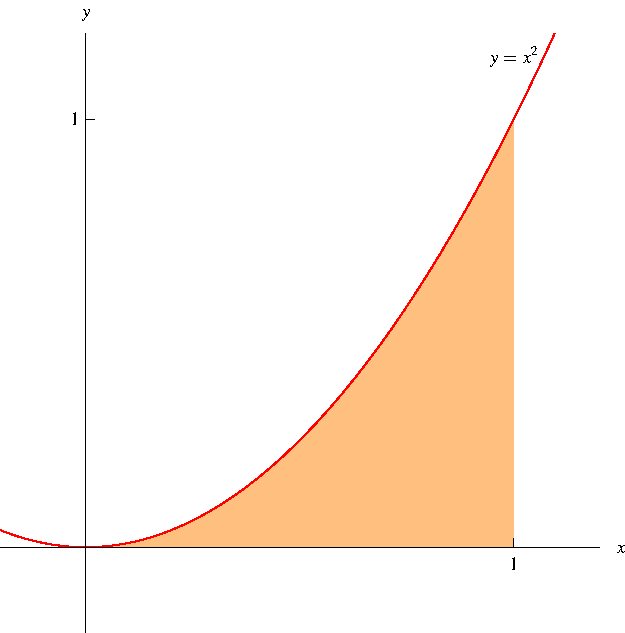
\includegraphics[height=4cm]{integration/pictures/05-01-xsquaredarea.pdf}%
%}}%
%\only<handout:6| 13>{%
%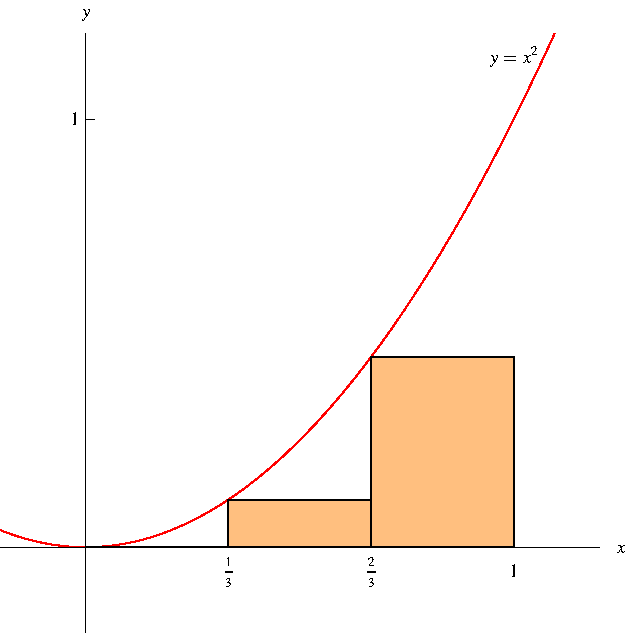
\includegraphics[height=4cm]{integration/pictures/05-01-lefta.pdf}%
%}%
%\only<handout:0| 14>{%
%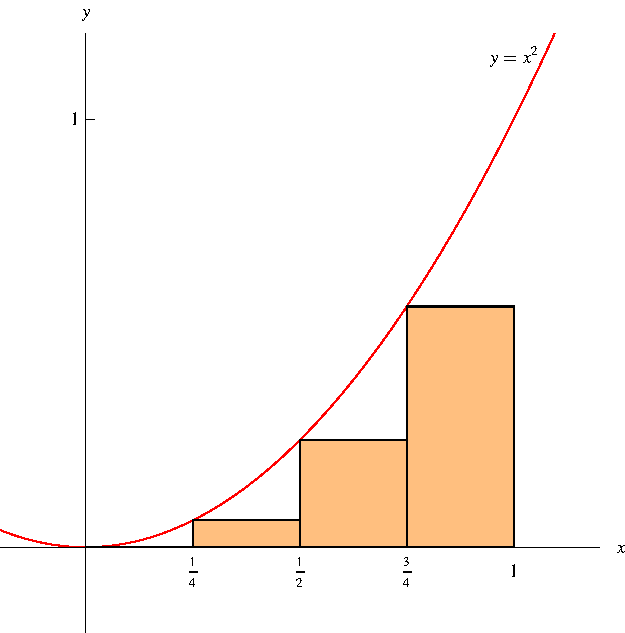
\includegraphics[height=4cm]{integration/pictures/05-01-leftb.pdf}%
%}%
%\only<handout:0| 15>{%
%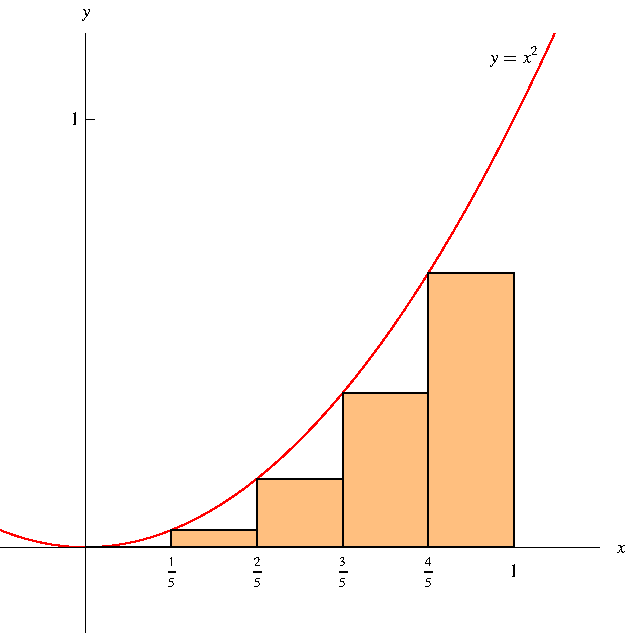
\includegraphics[height=4cm]{integration/pictures/05-01-leftc.pdf}%
%}%
%\only<handout:0| 16>{%
%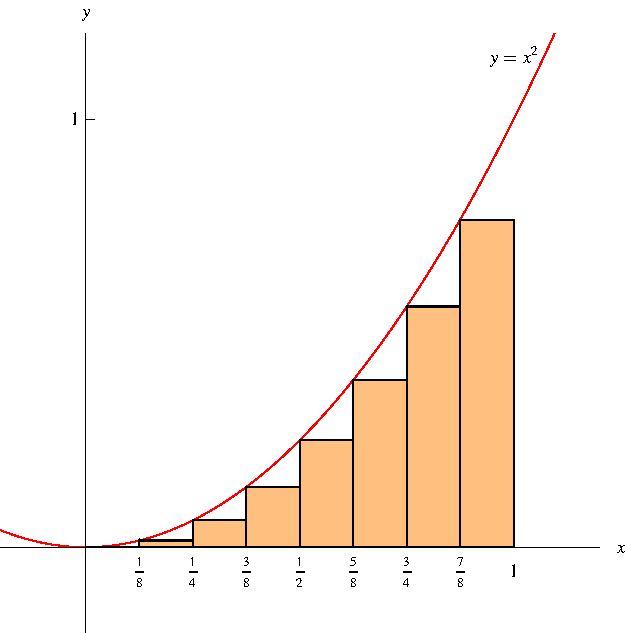
\includegraphics[height=4cm]{integration/pictures/05-01-leftd.pdf}%
%}%
%\only<handout:0| 17>{%
%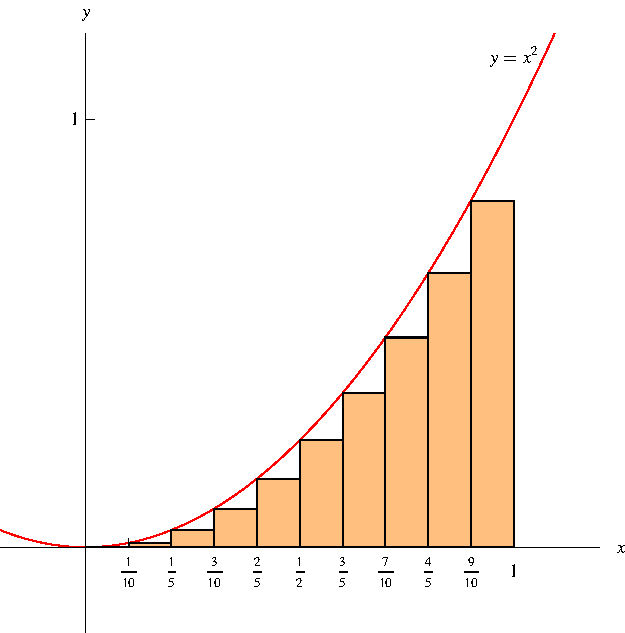
\includegraphics[height=4cm]{integration/pictures/05-01-lefte.pdf}%
%}%
%\only<handout:0| 18>{%
%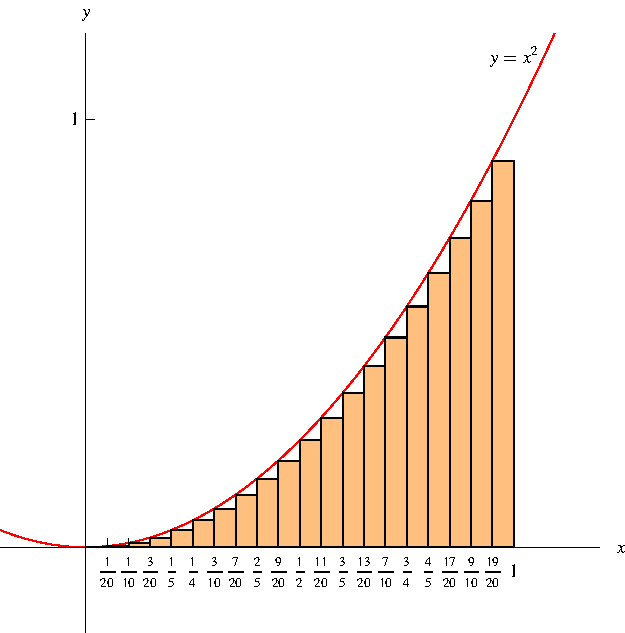
\includegraphics[height=4cm]{integration/pictures/05-01-leftf.pdf}%
%}%
%\only<handout:0| 19>{%
%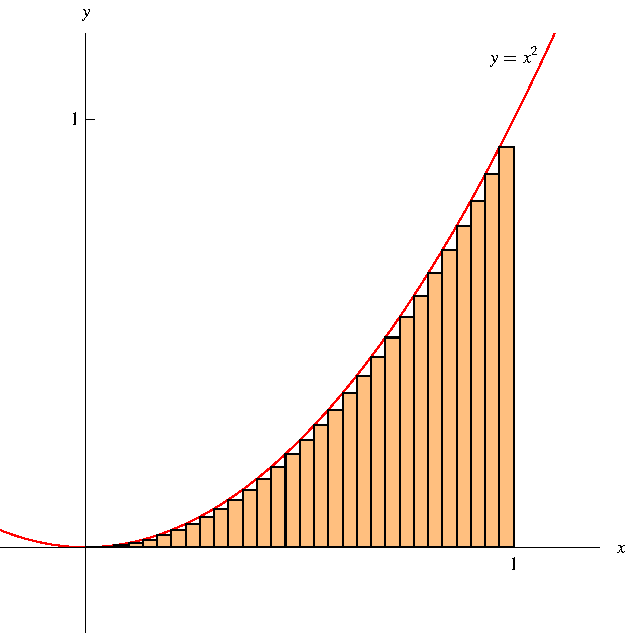
\includegraphics[height=4cm]{integration/pictures/05-01-leftg.pdf}%
%}%
%\only<handout:7| 20->{%
%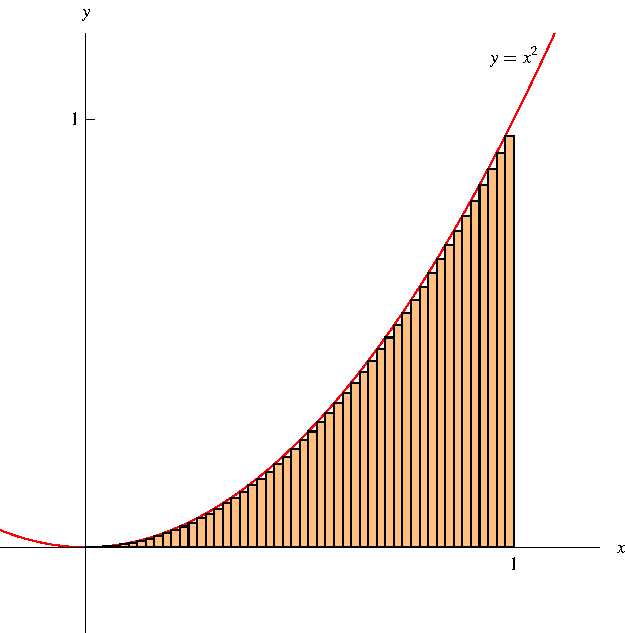
\includegraphics[height=4cm]{integration/pictures/05-01-lefth.pdf}%
%}%
%\ \only<handout:1| -2>{%
%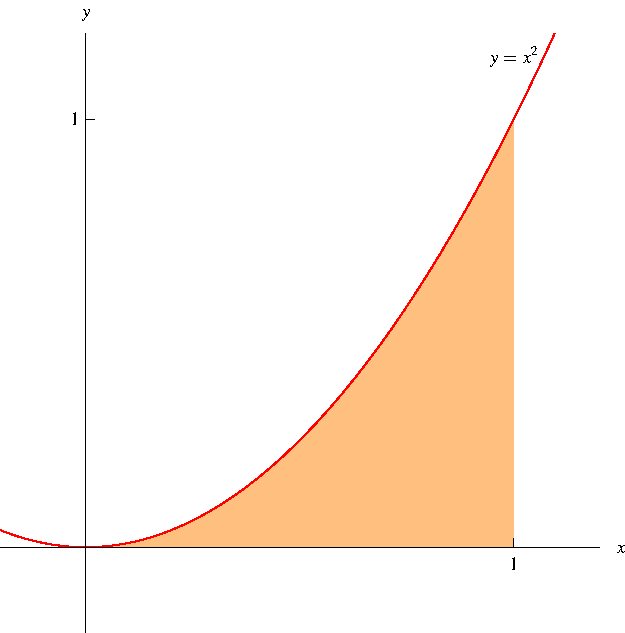
\includegraphics[height=4cm]{integration/pictures/05-01-xsquaredarea.pdf}%
%}%
%\only<handout:2| 3>{%
%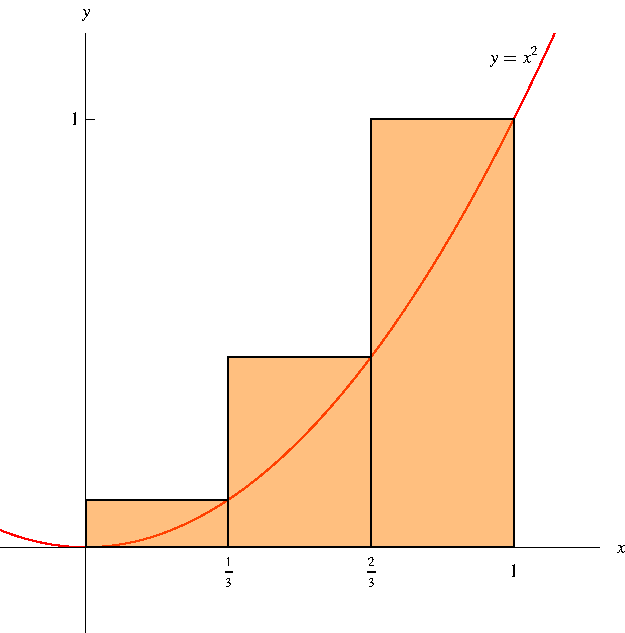
\includegraphics[height=4cm]{integration/pictures/05-01-righta.pdf}%
%}%
%\only<handout:3| 4>{%
%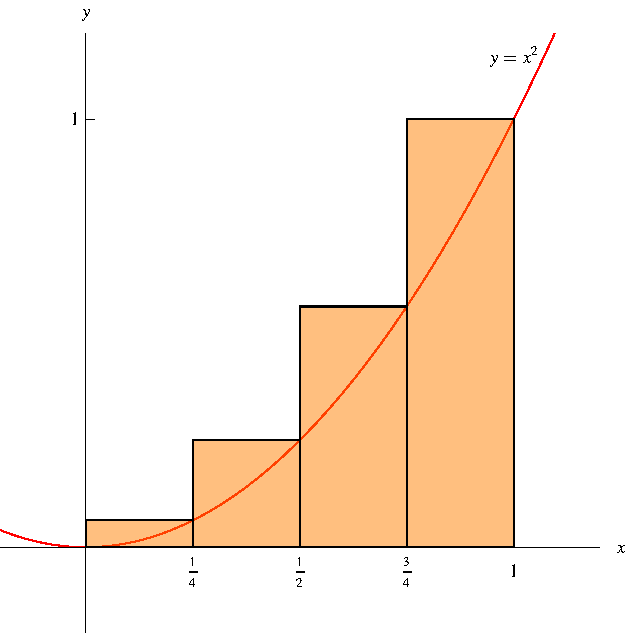
\includegraphics[height=4cm]{integration/pictures/05-01-rightb.pdf}%
%}%
%\only<handout:0| 5>{%
%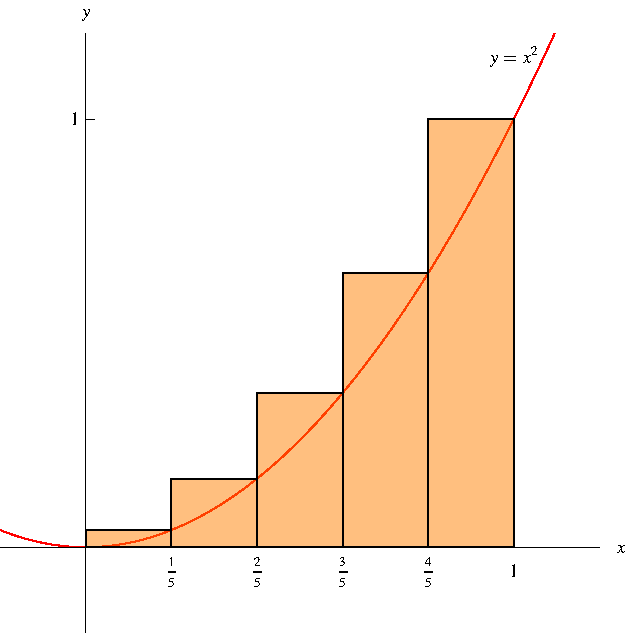
\includegraphics[height=4cm]{integration/pictures/05-01-rightc.pdf}%
%}%
%\only<handout:4| 6>{%
%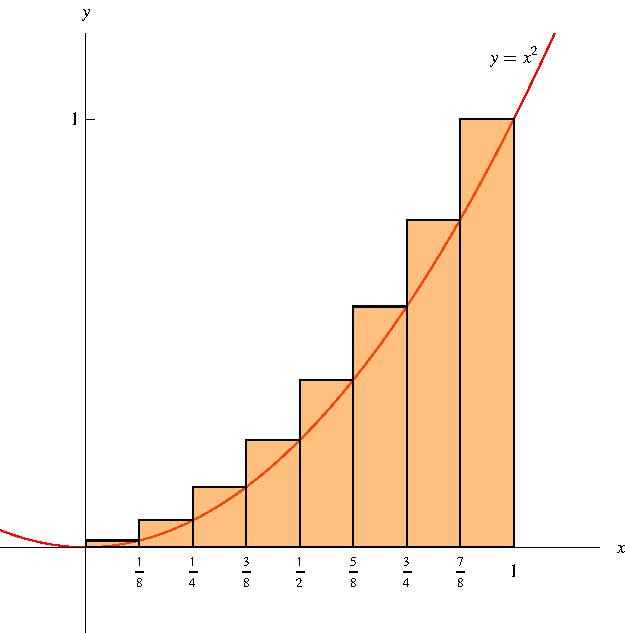
\includegraphics[height=4cm]{integration/pictures/05-01-rightd.pdf}%
%}%
%\only<handout:0| 7>{%
%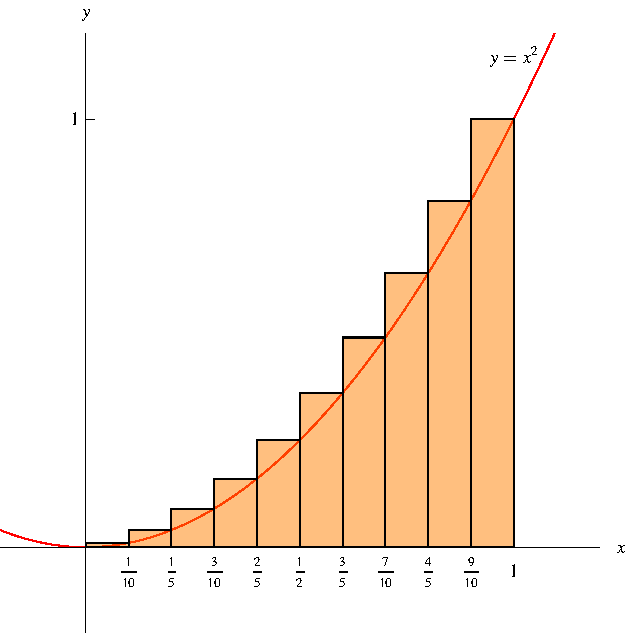
\includegraphics[height=4cm]{integration/pictures/05-01-righte.pdf}%
%}%
%\only<handout:0| 8>{%
%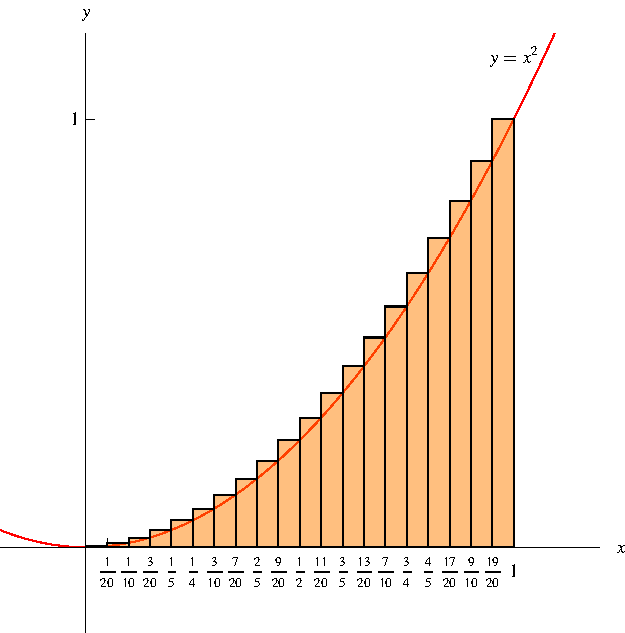
\includegraphics[height=4cm]{integration/pictures/05-01-rightf.pdf}%
%}%
%\only<handout:0| 9>{%
%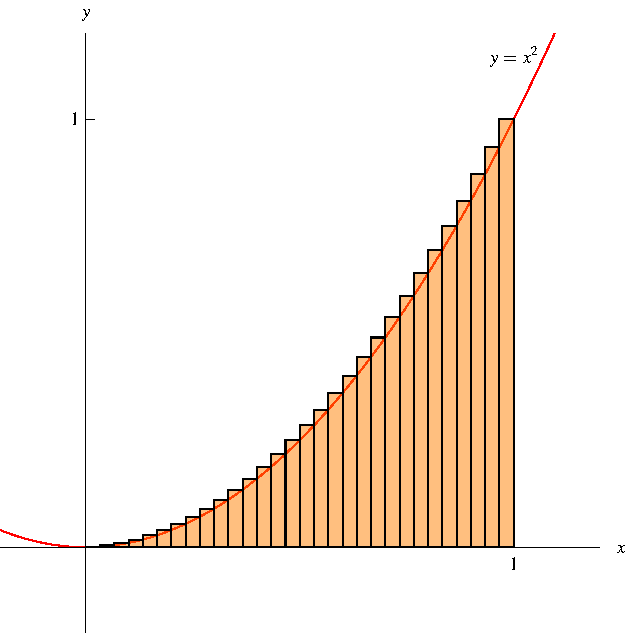
\includegraphics[height=4cm]{integration/pictures/05-01-rightg.pdf}%
%}%
%\only<handout:5-| 10->{%
%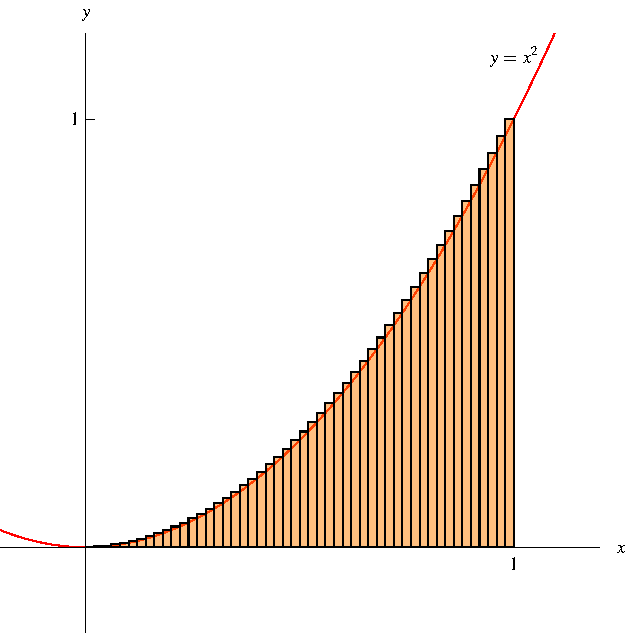
\includegraphics[height=4cm]{integration/pictures/05-01-righth.pdf}%
%}%
\end{center}
\end{frame}
% end module areas-intro

%begin module area-under-hyperbola-ex1

\begin{frame}
Recall Euler substitution: $x=\frac12\left(\frac{1}{t}- t \right)$, $\alert<2>{\sqrt{x^2+1}=\frac{1}2\left(\frac 1 t +t\right)}$, $\alert<12,13,14>{ t=\sqrt{x^2+1}-x} $, $\alert<3>{ \diff x=-\frac12 \left(\frac1{t^2} +1\right)\diff t}$.
\begin{example}
$
\begin{array}{rcl}
\displaystyle \int \alert<2>{ \sqrt{x^2+1}} \alert<3>{\diff x} \vphantom{ \frac{1}{8}\left(\frac{1}{ (\sqrt{ x^2 +1} -x)^2} - (\sqrt{x^2+1}- x)^2 \right) } &=&
\displaystyle
\only<1-16>{ 
\uncover<2->{ \alert<3>{-} \int  \alert<2>{\alert<4>{\frac12} \left(\alert<5,6>{\frac1t} +\alert<7,8>{t}\right)} \alert<3>{\alert<4>{ \frac{1}{2}} \left(\alert<5,7>{ \frac 1 {t^2}} +\alert<6,8>{1} \right)\diff t}} \\
\uncover<4->{ &=&\displaystyle -\alert<4>{ \frac 1 4} \alert<9,10,11>{ \int} \left(\alert<5>{ \alert<9>{ \frac{ 1 }{ t^3}}} + \alert<6,7,10>{2\frac{1}t} + \alert<8,11>{t} \right) \alert<9,10,11>{ \diff t} } \\
\uncover<9->{&=&\displaystyle \alert<15>{-\frac{1}4} \left(\alert<9>{\alert<15>{ -}\frac{ \alert<12>{ t^{-2}}}{\alert<15>{2}}} +\alert<10>{ \alert<15>{2} \ln\alert<14>{ |t|} }+ \alert<11>{\frac{\alert<13>{ t^2}}{\alert<15>{2}}} \right)+C}\\
\uncover<12->{&=&}
}
\uncover<12->{\displaystyle \only<1-24>{  \alert<16,18,24>{ \alert<15>{\frac{1}{8}} \left(\frac{1}{\alert<12>{ (\sqrt{ x^2 +1} -x)^2}} - \alert<13>{(\sqrt{x^2+1}- x)^2} \right) } }}\only<25->{
\alert<25>{ \frac{1}{2}x\sqrt{x^2+1}}
} {~~~~~~~~~~~~~~~~~~~~~~~~~~~~~~~~~~~~~~~~~~~~~~~~~~~~~~}  \\
\uncover<12->{ && \displaystyle \alert<16>{ \only<1-30>{\alert<15>{ -}} \only<31->{\alert<31>{+} } \alert<15>{ \frac12}  \alert<26,30>{\ln ( \alert<14>{ \sqrt{x^2+1} \only<1-30>{-}\only<31->{\alert<31>{+} } x})} +C}}
\end{array}
$

\noindent \only<17-25>{The answer is good. However, let's simplify.

\noindent 
\uncover<18->{
$
\begin{array}{l}
\phantom{=}
\displaystyle \alert<18>{ \frac{1}{(\sqrt{x^2+1}-x)^2}- ( \sqrt{ x^2+1 }-x)^2} \\
\uncover<19->{= \displaystyle \frac{ \alert<19>{(\sqrt{x^2+1} +x )^2} }{ ( \sqrt{x^2 +1} -x )^2  	\alert<19>{(\sqrt{x^2+1}+x)^2} } - (\sqrt{x^2+1}-x)^2} \\
\uncover<20->{ =\displaystyle \frac{(\sqrt{x^2+1}+x)^2}{ \alert<20>{ \alert<21,22>{((\sqrt{x^2 +1 } )^2 -x^2 )^2 } \uncover<21,22>{\alert<21,22>{=1}} } } - ( \sqrt{x^2 +1 } -x )^2} \\
\displaystyle \uncover<22->{=(\sqrt{x^2+1}+x)^2-( \sqrt{x^2 + 1 } -x)^2} \uncover<23->{ = \alert<24,25>{ 4x\sqrt{x^2+1}}}
\end{array}
$
} %uncover<18->
} %only<17-25>

\only<26->{
The last expression can be transformed to:
\[
\begin{array}{rcl}
\displaystyle 
\alert<26>{\ln} \left(\frac{\alert<26,28>{(\sqrt{x^2+1}-x)} \uncover<27->{ \alert<27,28>{( \sqrt{x^2+1}+ x )} }}{ \uncover<27->{ \alert<27>{ \sqrt{x^2 +1} +x}}} \right) 
&=& \displaystyle \uncover<28->{\alert<29>{ \ln \left( \frac{\alert<28>{ 1} }{ \sqrt{x^2+1}+x}\right)} }\\ \uncover<29->{&=&\alert<29,30,31>{ -\ln (\sqrt{x^2+1}+x)}}
\end{array}
\]
}
\end{example}

\vspace{8cm}
\end{frame}

\begin{frame}
\begin{example}
Find the area locked b-n the hyperbolas $\alert<2,3>{ y=\pm \sqrt{ x^2+1}}$ and $x=\pm 2\sqrt{ 2}$.
\begin{columns}
\column{.5\textwidth}
\psset{xunit=0.7cm, yunit=0.7cm}
\begin{pspicture}(-3.328427, -5)(3.328427,5) 
\psframe*[linecolor=white](-3.328427,-5)(3.328427,5) 
\tiny 
\uncover<31->{
\pscustom*[linecolor=\psColorAreaUnderGraph]{
\psplot[linecolor=\psColorGraph, plotpoints = 1000 ] {-2.828427} {2.828427}{1 x 2 exp add 0.5 exp }
\psline[linecolor=\psColorGraph](2.828427,-3)(2.828427,3)
\psplot[linecolor=\psColorGraph, plotpoints=1000] { 2.828427 } {-2.828427}{1 x 2 exp add 0.5 exp -1 mul }
\psline[linecolor=\psColorGraph](-2.828427,-3)(-2.828427,3)
}
}
\uncover<1-26,28->{
\psaxes[arrows=<->,ticks=none, labels=none](0,0)(-3,-3)(3,3) 
}
\psline[linecolor=red!1](3.301,2)(3.302,2)
\psline[linecolor=red!1](-3.301,2)(-3.302,2)

%Function formula: - (x^{2}+1)^{1/2} 
\psplot[linecolor=\psColorGraph, plotpoints=1000]{-2.828427}{2.828427}{1 x 2 exp add 0.5 exp -1 mul }
\uncover<3-4>{\rput[tl](-2.2, -2.4){ \alert<3>{ $y= - \sqrt{ x^2 +1 }$}}}

%Function formula: (x^{2}+1)^{1/2} 
\psplot[linecolor=\psColorGraph, plotpoints=1000]{-2.828427}{ 2.828427 }{1 x 2 exp add 0.5 exp }
\uncover<2-4>{\rput[bl](-2.1, 2.4){\alert<2>{ $y=\sqrt{ x^2 +1} $}}}

\uncover<29->{
\psline[linecolor=\psColorGraph](-2.828427,3)(-2.828427,-3)
}
\uncover<30->{
\psline[linecolor=\psColorGraph](2.828427,3)(2.828427,-3)
}
\uncover<25-27>{
\psline{<->}(-2.9,2.9)(2.9,-2.9)
\rput[t](-2.1, 1.7){$\begin{array}{l} \alert<25>{v=0} \\\uncover<1-26>{\alert<25>{y+x=0}} \end{array}$}
}
\uncover<15-27>{
\psline{<->}(-2.9,-2.9)(2.9,2.9)
\rput[b](-2.1, -1.9){$\begin{array}{l} \uncover<1-26>{ \alert<15>{ y-x=0 }}\\\uncover<16->{\alert<16>{u=0}} \end{array}$}
}
\uncover<17-26>{
\psFullDot{1.4}{1.4}
\rput[l]( 1.6, 1.4){$(\frac{y+x}{2},\frac{y+x}{2})$}
}
\uncover<14-26>{
\psFullDot{0.6}{2.2}
\rput[lb](0.65, 2.2){$(x,y)$}
}
\uncover<26>{
\psline(0.6,2.2)(-0.8,0.8)
\psline(-0.7, 0.9)(-0.6, 0.8)(-0.7, 0.7)
\rput[rb](-0.3, 1.3){\alert<26>{$v$}}
}
\uncover<18-26>{
\psline(0.6,2.2)(1.4, 1.4) 
\psline(1.3, 1.5)(1.2,1.4)(1.3, 1.3)
}
\uncover<23-26>{
\rput[tr](0.95, 1.8){\alert<23>{$u$}}
}
\uncover<14-26>{
\psFullDot{2.2}{0.6}
\rput[lt]( 2.2, 0.65){$(y,x)$}
}
\end{pspicture} 

\vbox to 3.0cm {
\uncover<18->{\alert<18>{
\uncover<22->{\alert<22>{Signed}} distance b-n $(x,y)$ and line $u=0$ equals}}
\only<1-23>{
$\uncover<19->{\uncover<22->{\alert<22>{\pm}} \alert<19>{ \sqrt{ \alert<20>{ \left(x-\frac{(x+y)}{2} \right)^2+ \left( y- \frac{(x+y )}{2} \right)^2}}}}
$
$\uncover<20->{=\uncover<22->{\alert<22>{\pm}} \sqrt{ \alert<20>{ \frac{1}{2}(y-x)^2 }}} \uncover<21->{= \alert<21>{ \uncover<1-21>{\pm} \alert<23>{ \frac{\sqrt{2 }}{ 2 } ( y-x)}}} \uncover<23>{ \alert<23>{=}}$
} %only<1-23>
\uncover<23->{ \alert<23,24>{$u $}.} 
\only<24->{\uncover<25->{
Similarly compute that \alert<26>{signed distance b-n $(x,y)$ and the \alert<25>{line $v=0$} equals $v$}. 
\uncover<27->{$\Rightarrow$ $y^2-x^2=1$ is the \alert<27>{ hyperbola $v=\frac{1/2}{v}$} in the $(u,v)$-plane.}
}}

\vfil
} %vbox 

\column {.5\textwidth}
\only<1-27>{
\uncover<4->{We studied $\alert<27>{v=\frac{1/2}{u}}$ is called a hyperbola:}\uncover<3->{ why do we call $y= \sqrt{ x^2 +1}$ hyperbola?} \uncover<5->{Compute:}
\[
\begin{array}{rcl}
\uncover<5->{\sqrt{x^2+1} &=& y}\\
\uncover<6->{ x^2+1 &=& y^2}\\
\uncover<7->{y^2-x^2&=&1}\\
\uncover<8->{\uncover<9>{\alert<9>{\frac{1}{2}}} \uncover<10->{\alert<10,11>{\frac{\sqrt{2}}{2}}} \alert<11>{(y-x)} \uncover<10->{\alert<10,12>{\frac{\sqrt{2}}{2}}} \alert<12>{(y+x)}&=&\uncover<9->{\alert<9>{\frac{1}{2}}} \uncover<8>{1}}\\
\uncover<11->{\alert<11>{u}\alert<12>{v}&=& \frac{1}{2}}\\
\uncover<13->{\alert<27>{v}&\alert<27>{=}& \alert<27>{\frac{1/2}{u}},}
\end{array}
\]
\uncover<11->{where $\begin{array}{|l}
\alert<11,16,23>{u=\frac{\sqrt{2}}{2} \left(y-x\right)}\\ 
\alert<12,25>{v=\frac{\sqrt{2}}{2}\left(y+x\right)}
\end{array}$. } \uncover<14->{Consider an arbitrary point $(x,y)$.}
} %only<1-27>
\only<28->{
The area in question is:
$
\begin{array}{l}
\displaystyle\phantom{=} \int \limits^{{{\uncover<28,29>{\alert<29>{ \textbf{?}}}\uncover<30->{\alert<30>{ 2\sqrt{2}}}}}}_{\uncover<28>{\alert<28>{\textbf{?}}}\uncover<29->{ -2\sqrt{2}}} 2\sqrt{x^2+1}\diff x \\
\displaystyle \uncover<32->{= \uncover<33->{\alert<33>{2}} \left[x\sqrt{x^2+1} \vphantom{\ln (\sqrt{x^2+1}+x)}\right.}\\
\displaystyle \uncover<32->{\left. \ln (\sqrt{x^2+1}+x)\right]^{2\sqrt{2}}_{\only<33->{\alert<33>{0}} \uncover<1-32>{-2\sqrt{2}}}}\\
\uncover<34->{=2\left(2\sqrt{2} \sqrt{(2\sqrt{2})^2+1}\right.} \\
\uncover<34->{\left.+ \ln (\sqrt{(2\sqrt{2})^2+1}+2\sqrt{2}) \right)}\\
\uncover<35->{=12\sqrt{2} +2\ln (3+2\sqrt{2})}\\
\uncover<36->{\approx 20.496}
\end{array}
$
}
\end{columns}

\end{example}

\end{frame}

%end module area-under-hyperbola-ex1
%begin module improper-integral-type1-arctan-geometric-interpretation
%\begin{comment}
\begin{frame}[t]

\psset{xunit=2cm, yunit=2cm}
\begin{pspicture}(-3.1, -0.1)(3.1,1.2) 
\psframe*[linecolor=white](-3.1,-0.1)(3.1,1.2) 
\tiny 
\psline[linecolor=red!1](0,1.2)(0.001,1.2) %bounding boxes don't always work right
\psaxes[arrows=<->, ticks=none, labels=none] (0,0) (-3.05,-0.1) (3.05,1.1)
\rput[t](3, -0.1){$x$}

%Function formula: - (- x^{2}+1)^{1/2} 
%\psplot[linecolor=\psColorGraph, plotpoints=1000]{-1}{1}{1 x 2 exp -1 mul add 0.5 exp -1 mul }
%Function formula: (- x^{2}+1)^{1/2} 
\psplot[linecolor=blue, plotpoints=1000] {-1} {1} {1 x 2 exp -1 mul add 0.5 exp }
\psline(-3,1)(3,1) 

\uncover<3->{
\psline{<-}(-0.05, 0)(-0.05,0.4)
\psline{->}(-0.05, 0.6)(-0.05,1)
\rput(-0.05, 0.5){\alert<3>{$1$}}
}
\uncover<2>{
\psline[linecolor=red](0.5,1)(1,1)
\psFullDot{1}{1}
}
\uncover<2>{
\psFullDot{0.5}{1}
}

\rput[br](-0.05, 1.05){ $\phantom{Q_0=P_0}A$}
\uncover<2->{
\rput[lb](0.5, 1.05){$P_1\phantom{(x_1 ,1)}$}
\rput[lb](1, 1.05){$P_2(\alert<2>{x_2}, 1)$}
}
\uncover<2->{
\rput[t](0.75,0.95){\alert<2>{$\Delta$}}
}
\uncover<5->{
\rput[lt](0.520000, 0.4500000){$\alert<5>{Q_2}$}
\rput[l](0.42000, 0.8){$\alert<5>{Q_1}$}
}
\rput[tl](0.05, -0.05){$O$}
%calculator commands:
%\Delta:=0.5;
%xInv{}{{x}}:=DoubleValue{}x/(1+x^2);
%yInv{}{{x}}:=DoubleValue{} 1/(1+x^2);
%xDir{}{{x}}:=-xInv{}x;
%yDir{}{{x}}:=1-yInv{}x;
%lengthN{}{{x}}:=((xDir{}x)^2+(yDir{}x)^2)^{1/2};
%xDirN{}{{x}}:=0.05 xDir{}x /lengthN{}x ;
%yDirN{}{{x}}:=0.05 yDir{}x/lengthN{}x;
%xT{}{{x}}:=-yDirN{}x;
%yT{}{{x}}:=xDirN{}x;

%inversePoint{}{{x}}:=(xInv{}x,yInv{}x );
%f{}{{x}}:= \psline(DoubleValue{}x,1 )(0,0) \psline inversePoint{}x (0,1)  \psline inversePoint{}x inversePoint{}(x+\Delta) \psline (xInv{}x +xDirN{}x, yInv{}x+yDirN{}x ) (xInv{}x +xDirN{}x+xT{}x, yInv{}x+yDirN{}x +yT{}x)(xInv{}x +xT{}x, yInv{}x +yT{}x);
%f{}(\Delta) f{}(2\Delta)f{}(3\Delta)f{}(4\Delta)f{}(5\Delta)f{}(6\Delta)

\uncover<5->{
\psline (0.5, 1) (0, 0) 
}
\uncover<5->{
\psline (0.4, 0.8) (0, 1) 
}
\uncover<15->{
\psline (0.4, 0.8) (0.5, 0.5) 
}
\uncover<5->{\psline (0.355279, 0.822361) (0.332918, 0.777639) (0.377639, 0.755279) }

\uncover<4->{\psline (1, 1) (0, 0) }
\uncover<5->{\psline (0.5, 0.5) (0, 1)} 
%\psline (0.5, 0.5) (0.461538, 0.307692) 
\uncover<5->{\psline (0.464645, 0.535355) (0.429289, 0.5) (0.464645, 0.464645) }


%\psline (1.500000, 1) (0, 0) 
%\psline (0.461538, 0.307692) (0, 1) 
%\psline (0.461538, 0.307692) (0.4, 0.2) 
%\psline (0.433803, 0.349295) (0.392201, 0.321560) (0.419936, 0.279957) 

%\psline (2, 1) (0, 0) 
%\psline (0.4, 0.2) (0, 1) 
%\psline (0.4, 0.2) (0.344828, 0.137931) 
%\psline (0.377639, 0.244721) (0.332918, 0.222361) (0.355279, 0.177639) 

%\psline (2.5, 1) (0, 0) 
%\psline (0.344828, 0.137931) (0, 1) 
%\psline (0.344828, 0.137931) (0.300000, 0.100000) 
%\psline (0.326258, 0.184355) (0.279834, 0.165785) (0.298404, 0.119362) 

%\psline (3, 1) (0, 0) 
%\psline (0.300000, 0.100000) (0, 1) 
%\psline (0.300000, 0.100000) (0.264151, 0.075472) 
%\psline (0.284189, 0.147434) (0.236754, 0.131623) (0.252566, 0.084189)

%\psline (-0.5, 1) (0, 0) 
%\psline (-0.4, 0.8) (0, 1) 
%\psline (-0.4, 0.8) (-0.5, 0.5) \psline (-0.355279, 0.822361) (-0.377639, 0.867082) (-0.422361, 0.844721) 

%\psline (-1, 1) (0, 0) 
%\psline (-0.5, 0.5) (0, 1) 
%\psline (-0.5, 0.5) (-0.461538, 0.307692) 
%\psline (-0.464645, 0.535355) (-0.5, 0.570711) (-0.535355, 0.535355) 

%\psline (-1.500000, 1) (0, 0) 
%\psline (-0.461538, 0.307692) (0, 1) 
%\psline (-0.461538, 0.307692) (-0.4, 0.2) 
%\psline (-0.433803, 0.349295) (-0.475406, 0.377030) (-0.503141, 0.335427) 

%\psline (-2, 1) (0, 0) 
%\psline (-0.4, 0.2) (0, 1) 
%\psline (-0.4, 0.2) (-0.344828, 0.137931) 
%\psline (-0.377639, 0.244721) (-0.422361, 0.267082) (-0.444721, 0.222361) 

%\psline (-2.5, 1) (0, 0) 
%\psline (-0.344828, 0.137931) (0, 1) 
%\psline (-0.344828, 0.137931) (-0.300000, 0.100000) 
%\psline (-0.326258, 0.184355) (-0.372682, 0.202924) (-0.391251, 0.156501) 

%\psline (-3, 1) (0, 0) 
%\psline (-0.300000, 0.100000) (0, 1) 
%\psline (-0.300000, 0.100000) (-0.264151, 0.075472) 
%\psline (-0.284189, 0.147434) (-0.331623, 0.163246) (-0.347434, 0.115811)


%Function formula: - (- x^{2}+1/4)^{1/2}+1/2 
%\psplot[linecolor=blue, plotpoints=1000]{-0.5}{0.5}{0.5 0.2500000 x 2 exp -1 mul add 0.5 exp -1 mul add }

%Function formula: (- x^{2}+1/4)^{1/2}+1/2 
%\psplot[linecolor=blue, plotpoints=1000]{-0.5}{0.5}{0.5 0.2500000 x 2 exp -1 mul add 0.5 exp add }

\uncover<3,6>{
\psline[linecolor=red](1, 1) (0, 0)(0,1)(1,1) 
}
\uncover<4>{
\psline[linecolor=red](0.5, 1) (0, 0)(0,1)(0.5,1) 
}

\uncover<7>{
\psline[linecolor=red](0.5, 0.5) (0, 0)(0,1)(0.5,0.5) 
}
\uncover<8>{
\psline[linecolor=green](0,0)(0,1)
\psline[linecolor=red](0,0)(1,1)
}
\uncover<9>{
\psline[linecolor=green](0,0)(0.5,0.5)
\psline[linecolor=red](0,0)(0,1)
}
\uncover<15>{
\psline[linecolor=red](0,0)(0.5, 0.5)(0.4,0.8)(0,0)
}
\uncover<16>{
\psline[linecolor=red](0,0)(1, 1)(0.5,1)(0,0)
}
\uncover<17,18>{
\psline[linecolor=green](0.5, 0.5)(0.4, 0.8) 
\psline[linecolor=red](0.5, 1)(1, 1) 
} 
\uncover<18>{
\psline[linecolor=green](0.5, 0.5)(0.0, 0.0) 
\psline[linecolor=red](0, 0)(0.5, 1) 
}
\end{pspicture}
\only<1-26>{
Draw a unit circle as above, let $O, A$ be as indicated. \uncover<2->{Let $P_2$ be the point $(\alert<2>{x_2},1)$, $P_1$ be the point $(x_2-\alert<2>{\Delta},1)$.} \uncover<3->{By the Pythagorean theorem, $\alert<25>{|OP_2|^2= 1 + x_2^2}$} \uncover<4->{and similarly $ |OP_1 |^2=1+(x_2-\Delta )^2$.} \uncover<5->{Let \alert<5>{$Q_1$}, \alert<5>{$Q_2$} be as indicated.} \uncover<6->{Then $\alert<6>{ \triangle OP_2A} $ is similar to $\alert<7>{\triangle OAQ_2} $.} \uncover<8->{By Euclidean geometry, $\alert<8>{ \frac{ \only<1-8>{{\color{green} |OA|}} \only<9->{|OA|} }{ |OP_2| }} =\alert<9>{ \frac{\only<9>{{\color{green}|OQ_2|}} \only<8,10->{|OQ_2|} }{|OA|}}$} \uncover<10->{ and so $\alert<12,24>{|OQ_2| |OP_2| }= |OA|^2 \alert<12,24>{ =1}$ \uncover<23->{ and therefore $\alert<23>{ \frac{|OQ_2|}{|OP_2|}} = \frac{ \alert<24>{|OQ_2| \alert<23>{| OP_2 |}} }{|OP_2|^{\alert<23>{2} }} \uncover<24->{= \frac{ \alert<24>{ 1} }{ \alert<25>{|OP_2|^2}} } \uncover<25->{ = \frac{1}{\alert<25>{ 1+x_2^2}}.}$}
} 
%The points $Q_2$, $P_2$ are often called ``inverse points w.r.t. the unit circle''.
\uncover<11->{Similarly conclude $\alert<13>{ |OQ_1|} \alert<14>{|OP_1|} =|OA|^2= \alert<12>{1} \uncover<12->{ \alert<12>{\alert<13,14>{=} \alert<14>{ |OQ_2|}\alert<13>{ |OP_2| }}.}$} 
\uncover<13->{Therefore $\alert<13>{ \frac{|OQ_1|}{  |OP_2|} } \alert<13,14>{=} \alert<14>{\frac{|OQ_2| }{ |OP_1|}} $} \uncover<15->{and so $ \alert<15>{\triangle OQ_2Q_1} $ is similar to $\alert<16>{\triangle OP_1P_2} $.} \uncover<17->{Therefore $\frac{ \only<17>{{\color{green}|Q_1Q_2|}} \only<18->{\alert<19>{ |Q_1Q_2|}} } { \alert<17,20>{|P_1P_2|} }= \alert<20>{ \frac{ \only<18>{\color{green}|OQ_2|} \only<1-17,19->{ |OQ_2|} }{ \alert<18>{|OP_1|} }}$} \uncover<19->{and so }
}
\uncover<19->{\alert<26,27>{\noindent $\alert<19>{|Q_1Q_2|} =\alert<20>{\frac{|P_1P_2| |OQ_2|} {|OP_1|}} \uncover<21->{=\left(\frac{\alert<21>{|OP_2|} }{|OP_1|}\right) \alert<23,24,25>{\frac{|OQ_2|} {\alert<21>{ |OP_2|}}} \alert<22>{ |P_1P_2|} } \uncover<22->{= \frac{|OP_2| } {|OP_1|} \frac{\alert<22>{ \Delta} }{\alert<23,24,25>{ 1+x_2^2}}.}$}}
\end{frame}
%\end{comment}
%\begin{comment}
\begin{frame}[t]
\psset{xunit=2cm, yunit=2cm}
\begin{pspicture}(-3.1, -0.1)(3.1,1.2) 
\psframe*[linecolor=white](-3.1,-0.1)(3.1,1.2) 
\tiny 
\psline[linecolor=red!1](0,1.2)(0.001,1.2) %bounding boxes don't always work right
\uncover<48->{
\pscustom*[linecolor=\psColorAreaUnderGraph]{
%Function formula: \frac{1}{x^{2}+1} 
\psplot[linecolor=\psColorGraph, plotpoints=1000]{-3.000000}{3.000000}{1.0000000 1.0000000 x 2.0000000 exp add div }
\psline(3.000000, 0)(-3.000000, 0)
}

%Function formula: \frac{1}{x^{2}+1} 
\psplot[linecolor=\psColorGraph, plotpoints=1000]{-3.000000} {3.000000} {1.0000000 1.0000000 x 2.0000000 exp add div }
}

\psaxes[arrows=<->, ticks=none, labels=none](0,0)(-3.05,-0.1)(3.05,1.1)
%Function formula: - (- x^{2}+1)^{1/2} 
%\psplot[linecolor=\psColorGraph, plotpoints=1000]{-1}{1}{1 x 2 exp -1 mul add 0.5 exp -1 mul }
%Function formula: (- x^{2}+1)^{1/2} 
\psplot[linecolor=blue, plotpoints=1000]{-1}{1}{1 x 2 exp -1 mul add 0.5 exp }
\psline(-3,1)(3,1) 
%calculator commands:
%\Delta:=0.5;
%xInv{}{{x}}:=DoubleValue{}x/(1+x^2);
%yInv{}{{x}}:=DoubleValue{} 1/(1+x^2);
%xDir{}{{x}}:=-xInv{}x;
%yDir{}{{x}}:=1-yInv{}x;
%lengthN{}{{x}}:=((xDir{}x)^2+(yDir{}x)^2)^{1/2};
%xDirN{}{{x}}:=0.05 xDir{}x /lengthN{}x ;
%yDirN{}{{x}}:=0.05 yDir{}x/lengthN{}x;
%xT{}{{x}}:=-yDirN{}x;
%yT{}{{x}}:=xDirN{}x;

%inversePoint{}{{x}}:=(xInv{}x,yInv{}x );
%f{}{{x}}:= \psline(DoubleValue{}x,1 )(0,0) \psline inversePoint{}x (0,1)  \psline inversePoint{}x inversePoint{}(x+\Delta) \psline (xInv{}x +xDirN{}x, yInv{}x+yDirN{}x ) (xInv{}x +xDirN{}x+xT{}x, yInv{}x+yDirN{}x +yT{}x)(xInv{}x +xT{}x, yInv{}x +yT{}x);
%f{}(\Delta) f{}(2\Delta)f{}(3\Delta)f{}(4\Delta)f{}(5\Delta)f{}(6\Delta)

\uncover<1-33>{
\psline(0.5, 1)(0, 0)
}
\uncover<34-41>{
\psline(0.4, 0.8)(0, 0)
} 
\psline(0.4, 0.8)(0, 1) 
\uncover<28,34>{
\psline[linecolor=red](0.4, 0.8)(0, 1) 
}
\uncover<1-41>{
\psline(0.355279, 0.822361)(0.332918, 0.777639)(0.377639, 0.755279) 
}
\uncover<22>{
\psline[linecolor=red](0.4, 0.8)(0, 1) 
\psline[linecolor=red](0.355279, 0.822361)(0.332918, 0.777639)(0.377639, 0.755279) 
}
\uncover<7-12>{
\psline(0.600000, 1)(0, 0) 
\psline(0.441176, 0.735294)(0, 1) 
\psline(0.441176, 0.735294)(0.4, 0.8) 
\psline(0.398302, 0.761019)(0.372577, 0.718144)(0.415452, 0.692419) 
}
\rput[lt](0.46, 0.71){\uncover<7-12>{$Q_2$}}
\uncover<6>{
\psline(0.700000, 1)(0, 0) 
\psline(0.469799, 0.671141)(0, 1) 
\psline(0.469799, 0.671141)(0.4, 0.8)
\psline(0.428837, 0.699814)(0.400164, 0.658852)(0.441126, 0.630179)
}
\rput[lt](0.48, 0.65){\uncover<6>{$Q_2$}}
\uncover<5>{
\psline(0.8, 1)(0, 0) 
\psline(0.487805, 0.609756)(0, 1) 
\psline(0.487805, 0.609756)(0.4, 0.8)
\psline(0.448761, 0.640991)(0.417527, 0.601947)(0.456570, 0.570713) 
}
\rput[lt](0.5, 0.58){\uncover<5>{$Q_2$}}
\uncover<4>{
\psline(0.900000, 1) (0, 0) 
\psline(0.497238, 0.552486)(0, 1) 
\psline(0.497238, 0.552486)(0.4, 0.8)
\psline(0.460073, 0.585934)(0.426625, 0.548770)(0.463789, 0.515321)
}
\rput[lt](0.5, 0.54){\uncover<4>{$Q_2$}}

\uncover<1-3>{ %
\psline(1, 1)(0, 0) 
\psline(0.4, 0.8)(0.5, 0.5) 
} %
\rput[lt](0.520000, 0.4500000){\uncover<1-3>{$Q_2$}}
\uncover<13->{ %
\psline(0.4, 0.8)(0.5, 0.5) 
} %
\rput[lt](0.520000, 0.4500000){\uncover<13->{$Q_2$}}
\uncover<13-33>{ %
\psline(1, 1)(0, 0)
} 
\uncover<34-41>{
\psline(0.5, 0.5)(0, 0)
}
\uncover<30,34>{
\psline[linecolor=red](0.4, 0.8)(0.5, 0.5) 
}
\uncover<32->{
\psline(0.5, 0.5)(0.461538, 0.307692)
}
\uncover<32,34>{
\psline[linecolor=red](0.5, 0.5)(0.461538, 0.307692)
}
\uncover<1-3, 13-41>{
\psline(0.5, 0.5)(0, 1) 
\psline(0.464645, 0.535355)(0.429289, 0.5)(0.464645, 0.464645) 
}
\uncover<23>{
\psline[linecolor=red](0.5, 0.5)(0, 1) 
\psline[linecolor=red](0.464645, 0.535355)(0.429289, 0.5)(0.464645, 0.464645) 
}
\uncover<14>{ %
\psline[linecolor=red](0,0)(0,1)
} %
\uncover<15>{
\psline[linecolor=red](0,0)(0.5,1)
}
\uncover<16>{
\psline[linecolor=red](0,0)(1,1)
}
\uncover<17-33>{
\psline(1.5, 1)(0, 0) 
}
\uncover<34-41>{
\psline(0.461538, 0.307692)(0, 0) 
}
\uncover<17>{
\psline[linecolor=red](1.500000, 1)(0, 0) 
}
\uncover<32->{
\psline(0.461538, 0.307692)(0.4, 0.2) 
}
\uncover<32,34>{
\psline[linecolor=red](0.461538, 0.307692)(0.4, 0.2) 
}
\uncover<24-41>{
\psline(0.461538, 0.307692)(0, 1) 
\psline(0.433803, 0.349295)(0.392201, 0.321560)(0.419936, 0.279957) 
}
\uncover<24>{
\psline[linecolor=red](0.461538, 0.307692)(0, 1) 
\psline[linecolor=red](0.433803, 0.349295)(0.392201, 0.321560)(0.419936, 0.279957) 
}
\uncover<18-33>{ 
\psline(2, 1)(0, 0) 
}
\uncover<34-41>{
\psline(0.4, 0.2)(0, 0) 
}
\uncover<18>{ 
\psline[linecolor=red](2, 1)(0, 0) 
}
\uncover<32->{
\psline(0.4, 0.2)(0.344828, 0.137931) 
}
\uncover<32,34>{
\psline[linecolor=red](0.4, 0.2)(0.344828, 0.137931) 
}
\uncover<25-41>{
\psline(0.4, 0.2)(0, 1) 
\psline(0.377639, 0.244721)(0.332918, 0.222361)(0.355279, 0.177639) 
}
\uncover<25>{
\psline[linecolor=red](0.4, 0.2)(0, 1) 
\psline[linecolor=red](0.377639, 0.244721)(0.332918, 0.222361)(0.355279, 0.177639) 
}
\uncover<19-33>{ 
\psline(2.5, 1)(0, 0) 
}
\uncover<34-41>{ 
\psline(0.344828, 0.137931)(0, 0) 
}
\uncover<19>{ 
\psline[linecolor=red](2.5, 1)(0, 0)
}
\uncover<32->{
\psline(0.344828, 0.137931)(0.300000, 0.100000) 
}
\uncover<32,33,34>{
\psline[linecolor=red](0.344828, 0.137931)(0.300000, 0.100000) 
}
\uncover<26-41>{
\psline(0.344828, 0.137931)(0, 1) 
\psline(0.326258, 0.184355)(0.279834, 0.165785)(0.298404, 0.119362) 
}
\uncover<26>{
\psline[linecolor=red](0.344828, 0.137931)(0, 1) 
\psline[linecolor=red](0.326258, 0.184355)(0.279834, 0.165785)(0.298404, 0.119362) 
}
\uncover<20-33>{ 
\psline(3, 1)(0, 0) 
}
\uncover<34-41>{
\psline(0.300000, 0.100000)(0, 0) 
}
\uncover<20>{ 
\psline[linecolor=red](3, 1)(0, 0) 
}
%\psline(0.300000, 0.100000)(0.264151, 0.075472) 
\uncover<27-41>{
\psline(0.300000, 0.100000)(0, 1) 
\psline(0.284189, 0.147434)(0.236754, 0.131623)(0.252566, 0.084189)
}
\uncover<27->{
\rput[lt](0.3,0.095){$Q_n$}
}
\uncover<27>{
\psline[linecolor=red](0.300000, 0.100000)(0, 1) 
\psline[linecolor=red](0.284189, 0.147434)(0.236754, 0.131623)(0.252566, 0.084189)
}

\uncover<44>{
\psline(-0.5, 1)(0, 0) 
\psline(-0.4, 0.8)(0, 1) 
\psline(-0.355279, 0.822361)(-0.377639, 0.867082)(-0.422361, 0.844721) 

\psline(-1, 1)(0, 0) 
\psline(-0.5, 0.5)(0, 1) 
\psline(-0.464645, 0.535355)(-0.5, 0.570711)(-0.535355, 0.535355) 

\psline(-1.500000, 1) (0, 0) 
\psline(-0.461538, 0.307692)(0, 1) 
\psline(-0.433803, 0.349295)(-0.475406, 0.377030)(-0.503141, 0.335427) 

\psline(-2, 1) (0, 0) 
\psline(-0.4, 0.2)(0, 1) 
\psline(-0.377639, 0.244721)(-0.422361, 0.267082)(-0.444721, 0.222361) 

\psline(-2.5, 1) (0, 0) 
\psline(-0.344828, 0.137931)(0, 1) 
\psline(-0.326258, 0.184355)(-0.372682, 0.202924)(-0.391251, 0.156501) 

\psline(-3, 1)(0, 0) 
\psline(-0.300000, 0.100000)(0, 1) 
%\psline (-0.300000, 0.100000) (-0.264151, 0.075472) 
\psline(-0.284189, 0.147434)(-0.331623, 0.163246)(-0.347434, 0.115811)
}
\uncover<44->{
\psline(-0.4, 0.8)(-0.5, 0.5) 
\psline(-0.5, 0.5)(-0.461538, 0.307692) 
\psline(-0.461538, 0.307692)(-0.4, 0.2) 
\psline(-0.4, 0.2)(-0.344828, 0.137931) 
\psline(-0.344828, 0.137931)(-0.300000, 0.100000) 
}

%Function formula: - (- x^{2}+1/4)^{1/2}+1/2 
\uncover<42->{\psplot[linecolor=red, plotpoints=1000]{-0.5}{0.5}{0.5 0.2500000 x 2 exp -1 mul add 0.5 exp -1 mul add }

%Function formula: (- x^{2}+1/4)^{1/2}+1/2 
\psplot[linecolor=red, plotpoints=1000]{-0.5}{0.5}{0.5 0.2500000 x 2 exp -1 mul add 0.5 exp add }
}
\uncover<8-12>{
\psline[linecolor=red](0,0)(0.6,1)
\psline[linecolor=green](0,0)(0.5,1)
}
\uncover<4>{
\rput[lb](0.9, 1.05){$P_2$}
\rput[t](0.7,0.95){$\Delta$}
}
\uncover<5>{
\rput[lb](0.8, 1.05){$P_2$}
\rput[t](0.65,0.95){$\Delta$}
}
\uncover<6>{
\rput[lb](0.7, 1.05){$P_2$}
\rput[t](0.6,0.95){$\Delta$}
}
\uncover<7-12>{
\rput[lb](0.6, 1.05){$P_2$}
\rput[t](0.55,0.95){$\Delta$}
}
\uncover<1-3,13->{
\rput[lb](1, 1.05){\uncover<1-33>{$P_2\alert<16>{(x_2, 1)}$}}
\rput[t](0.75,0.95){$\Delta$}
}
\rput[rb](3, 1.05){$\uncover<20-33>{\alert<20>{P_n}}$}
\rput[lb](2, 1.05){
$\uncover<17-33>{\alert<17>{\dots}}$
}

\rput[lb](0.5, 1.05){\uncover<1-33>{$P_1\uncover<15->{\alert<15>{(x_1 ,1)}}$}}
\rput[t](3, -0.1){$x$}
\rput[br](-0.05, 1.05){$\uncover<21->{\alert<21>{Q_0= }}\uncover<14->{ \alert<14>{ P_0=}}A$}
\rput[l](0.42000, 0.8){$Q_1$}
\rput[tl](0.05, -0.05){$O$}
\end{pspicture}
\alert<1>{ \noindent $\alert<28>{|Q_1Q_2| =} \alert<29>{\frac{|OP_2| } {|OP_1|}} \alert<28>{\frac{ \Delta} {1+x_2^2}}. \vphantom{={\frac{|P_1P_2| |OQ_2|} {|OP_1|}} {=\left(\frac{|OP_2|}{|OP_1|}\right) \frac{|OQ_2|} { |OP_2|} |P_1P_2| } }$} \uncover<13->{For any $\varepsilon >0$, can choose $\Delta$: $\alert<29>{1< \frac{|OP_2| } {|OP_1|} < 1 + \varepsilon}$.}

\only<1-12>{ \uncover<2->{If we let $P_2\to P_1$}\uncover<3->{, i.e., $\Delta \to 0$,} \uncover<8->{we get $\alert<8>{ \frac{|OP_2| }{ |OP_1|}\to 1}$.} \uncover<9->{In strict mathematical language: for every $\varepsilon>0$ there exists $\delta >0$ such that when $\Delta  < \delta$ we have that $1>\frac{ |OP_2| }{|OP_1|}>1-\varepsilon $.} \uncover<10->{Furthermore, the choice of $\delta$ can be made independent of the value of $x_2$: } \uncover<11->{to prove that one analyzes the expression $\frac{|OP_2|}{|OP_1|} = \sqrt{ \frac{ 1+x_2^2} { 1 + (x_2-\Delta )^2}}$.} \uncover<12->{We leave the tedious but otherwise easy details to the interested student. } 
}

\only<13-27>{
\uncover<13->{Fix a large number $N$ and let $\Delta$ be such that $n= \frac{N}{\Delta} $ is integer.} \uncover<14->{ Let  $\alert<14>{P_0=(0,1)} $, $\alert<15>{P_1=(\Delta, 1 )}$, $\alert<16>{P_2=(2\Delta,1)}, \dots, \alert<20>{P_n= (n \Delta,1)}$}\uncover<21->{, and let $\alert<21>{Q_0}, \alert<22>{ Q_1},\alert<23>{Q_2}, \dots, \alert<27>{Q_n}$ be as indicated.} 
}

\uncover<28->{
$
\begin{array}{rcrcl}
\only<1-39>{
\alert<28>{ \frac{\Delta}{1+x_1^2 } }&<\phantom{=}&\alert<28>{ |Q_0Q_1|} &< \phantom{=} & \alert<29>{ (1+ \varepsilon )} \alert<28>{\frac{ \Delta}{1+x_1^2}}  \\
\uncover<30->{\alert<30>{ \frac{\Delta}{1+x_2^2 }} &<\phantom{=} &\alert<30>{|Q_1Q_2|} &<\phantom{=} & \alert<31>{ (1 + \varepsilon)} \alert<30>{\frac{ \Delta }{1+ x_2^2}}}  \\
\uncover<32->{ &\alert<32>{\vdots}} \\
\uncover<33->{\frac{\Delta}{1+x_n^2 } &<\phantom{=} &\alert<33>{ |Q_{n-1}Q_n|} &< \phantom{=} &(1+\varepsilon) \frac{\Delta}{1+x_n^2}} \uncover<34->{\\ \hline} 
\uncover<34->{ \sum_{i=1}^n\frac{\Delta}{1+x_i^2 } &< \phantom{=}&\alert<34>{ \sum_{i=1}^n |Q_{i-1} Q_i|} & <\phantom{=}& (1 +\varepsilon)\sum_{i=1}^n \frac{\Delta}{1+x_i^2} }\\
\uncover<35->{ \downarrow  &&\downarrow&&\downarrow}\\
}
\uncover<35->{ \alert<39,40>{\int_{0}^{\uncover<37->{\alert<37>{\infty}} \uncover<35,36>{N}} \frac{\diff x}{1+x^2}} & \uncover<1-38>{<} \uncover<39->{\alert<39,40>{=}}& \alert<39,40>{  \lim\limits_{\Delta\uncover<37->{, \alert<37>{N} }\uncover<39->{, \alert<39>{\varepsilon}}} \sum| Q_{i-1} Q_i|} \uncover<1-39>{ &\uncover<1-38>{<} \uncover<39->{\alert<39>{=}}& \uncover<1-38>{(1 + \varepsilon )} \int_0^{\uncover<37->{\alert<37>{\infty}} \uncover<35,36>{ N}} \frac{ \diff x}{1+x^2}}}
\end{array}
$
}

\only<1-39>{
\uncover<35->{Let $\Delta\to 0$.} \uncover<36->{Next take $\alert<36,37>{N\to \infty}$.} \uncover<38->{Finally take \alert<38,39>{$\varepsilon\to 0$}\uncover<39->{, use squeeze thm.}} 
}

\uncover<41->{
The points $Q_1, Q_2, \dots$ see the segment $OA$ from an angle of $\frac{\pi}{2}$. }\uncover<42->{Therefore, by Euclidean geometry, the points $Q_1, Q_2,\dots $ lie on the circle $C$ with radius $\frac{1}{2}$ and center $(0,\frac{1}{2}) $. } \uncover<43->{Therefore $ \sum |Q_{i-1}Q_{i}| $ approximates half of the circumference of the circle $C$.} 
\uncover<44->{\alert<44,45>{By symmetry,}
\uncover<46->{
\[
\alert<47>{\int_{-\infty}^{\infty} \frac{\diff x}{1+x^2} }= \text{ circumference of }C  \uncover<47->{=2\pi \left(\frac{1}{2}\right) \alert<47>{=\pi},}
\] 
\uncover<47,48->{as desired.}
}
}
\end{frame}
%\end{comment}
\begin{comment}
\begin{frame}[t]
\psset{xunit=2cm, yunit=2cm}
\begin{pspicture}(-3.1, -0.1)(3.1,1.2) 
\psframe*[linecolor=white](-3.1,-0.1)(3.1,1.2) 
\tiny 
%\psline[linecolor=red!1](0,1.2)(0.001,1.2) %bounding boxes don't always work right
%\pscustom*[linecolor=\psColorAreaUnderGraph]{
%Function formula: \frac{1}{x^{2}+1} 
%\psplot[linecolor=\psColorGraph, plotpoints=1000]{-3.000000}{3.000000}{1.0000000 1.0000000 x 2.0000000 exp add div }
%\psline(3.000000, 0)(-3.000000, 0)
%}

%Function formula: \frac{1}{x^{2}+1} 
%\psplot[linecolor=\psColorGraph, plotpoints=1000]{-3.000000} {3.000000} {1.0000000 1.0000000 x 2.0000000 exp add div }

\psaxes[arrows=<->, ticks=none, labels=none](0,0)(-3.05,-0.1)(3.05,1.1)
%Function formula: - (- x^{2}+1)^{1/2} 
%\psplot[linecolor=\psColorGraph, plotpoints=1000]{-1}{1}{1 x 2 exp -1 mul add 0.5 exp -1 mul }
%Function formula: (- x^{2}+1)^{1/2} 
\psplot[linecolor=blue, plotpoints=1000]{-1}{1}{1 x 2 exp -1 mul add 0.5 exp}
\psline(-3,1)(3,1) 

%Function formula: - (- x^{2}+1/4)^{1/2}+1/2 
\psplot[linecolor=red, plotpoints=1000] {-0.5}{0.5}{0.5 0.2500000 x 2 exp -1 mul add 0.5 exp -1 mul add }
%Function formula: (- x^{2}+1/4)^{1/2}+1/2 
\psplot[linecolor=red, plotpoints=1000]{-0.5}{0.5}{0.5 0.2500000 x 2 exp -1 mul add 0.5 exp add }


%calculator commands:
%\Delta:=0.5;
%xInv{}{{x}}:=DoubleValue{}x/(1+x^2);
%yInv{}{{x}}:=DoubleValue{} 1/(1+x^2);
%xDir{}{{x}}:=-xInv{}x;
%yDir{}{{x}}:=1-yInv{}x;
%lengthN{}{{x}}:=((xDir{}x)^2+(yDir{}x)^2)^{1/2};
%xDirN{}{{x}}:=0.05 xDir{}x /lengthN{}x ;
%yDirN{}{{x}}:=0.05 yDir{}x/lengthN{}x;
%xT{}{{x}}:=-yDirN{}x;
%yT{}{{x}}:=xDirN{}x;

%inversePoint{}{{x}}:=(xInv{}x,yInv{}x );
%f{}{{x}}:= \psline(DoubleValue{}x,1 )(0,0) \psline inversePoint{}x (0,1)  \psline inversePoint{}x inversePoint{}(x+\Delta) \psline (xInv{}x +xDirN{}x, yInv{}x+yDirN{}x ) (xInv{}x +xDirN{}x+xT{}x, yInv{}x+yDirN{}x +yT{}x)(xInv{}x +xT{}x, yInv{}x +yT{}x);
%f{}(\Delta) f{}(2\Delta)f{}(3\Delta)f{}(4\Delta)f{}(5\Delta)f{}(6\Delta)

\psline(0.5, 1)(0, 0)
\psline(0.4, 0.8)(0, 0)

\psline(1, 1)(0, 0) 
\psline(0.4, 0.8)(0.5, 0.5)
\psline[linecolor=red](0.4, 0.8)(0.5, 0.5) 
\psline(0.5, 0.5)(0, 0)

\psline(0.5,0)(0.5,0.316228)(1, 0.316228)(1,0)
\psline[linecolor=red](0.5,0 )(0.5,0.316228)


\rput[lb](1, 1.05){$P_2(x_2, 1)$}
\rput[t](0.75,0.95){$\Delta$}

\rput[lb](0.5, 1.05) {  $P_1  (x_1 ,1)$}
\rput[t](3, -0.1){$x$}
\rput[lt](0.520000, 0.4500000){$Q_2$}
\rput[l](0.42000, 0.8){$Q_1$}
\rput[tl](0.05, -0.05){$O$}
\end{pspicture}

We finish with illustration of the integral $\int_{-\infty}^{\infty} \frac{1}{1+x^2}\diff x $. Recall $|Q_1Q_2|\approx \frac{\Delta}{1+x_2^2} $. 

\end{frame}
\end{comment}
%end module improper-integral-type1-arctan-geometric-interpretation

\begin{frame}
\begin{example}
A cone is folded from a wedge-shaped profile of radius $r$. Find the maximal possible volume $V$ of such a cone.

\begin{columns}[c]
\column{.27\textwidth}
%Please note: the below pictures are up to scale. The cone is an isogonal projection onto the tangent plane to the sphere centered at the origin and passing through point (0, 2, 0.4). The function used to draw the cone is 
%the vector partition calculator function plotConeUsualProjection(3/4, \sqrt(1-DoubleValue{}(3/4)^2), 2, 0.4)
\psset{xunit=1.5cm, yunit=1.5cm}
\begin{pspicture}(-5, -5)(5,5) 
\psframe*[linecolor=white](-5,-5)(5,5) 
\tiny 
\pscustom*[linecolor=cyan!30]{ \psparametricplot[algebraic] {2.35619}{7.06858} {0+1*cos(t)| 0+1*sin(t)} \psline(0.707107, 0.707107)(0, 0)(-0.707107, 0.707107)}

\psparametricplot[algebraic,linecolor=blue]{2.35619}{7.06858}{cos(t)| sin(t)} 
\psline[linecolor=red](0.707107, 0.707107)(0, 0)(-0.707107, 0.707107)

\rput[t](0.35, 0.30){$r$}
\rput[lb](0.8,0.8){$B$}
\rput[rb](-0.8,0.8){$A$}
\rput[b](0,0.1){$O$}

\uncover<7->{
\psparametricplot[algebraic,linecolor=purple]{2.35619}{7.06858}{0.07*cos(t)| 0.07*sin(t)} 
\rput[t](0, -0.1){$\alert<7>{\theta}$}
}
\uncover<8->{
\psparametricplot[linewidth=1pt, algebraic,arrows=<->, linecolor =blue] {4.41238898} {5.01238898}{cos(t)| sin(t)} 
}
\uncover<9->{
\rput[b](0, -0.9){\alert<9>{$r\theta$}}
}
\psline[linecolor=red!1](-1.03,-1.03)(-1.03,-1.02)
\end{pspicture} 

\psset{xunit=1.5cm, yunit=1.5cm}
\begin{pspicture}(-5, -5)(5,5) 
\psframe*[linecolor=white](-5,-5)(5,5) 
\tiny 
\rput[b](0,0.7){$O$}
\rput[l](0.8, 0.0333562){$A$}

\psline[linecolor=\psColorGraph](0.73046, 0.0333562)(0, 0.648593)
\psline[linecolor=\psColorGraph](-0.73046, 0.0333562)(0, 0.648593)
\psparametricplot[algebraic,linecolor=blue]{-3.37036}{0.228769}{0.75*cos(t) |0.147087*sin(t)}
\psparametricplot[algebraic, linestyle=dashed, linecolor=blue] {0.228769}{2.91282}{0.75*cos(t) |0.147087*sin(t)}
\rput[bl](0.38,0.34 ){$r$}

\uncover<10,11>{
\psparametricplot[algebraic,linecolor=red]{-3.37036}{0.228769}{0.75*cos(t) |0.147087*sin(t)}
\psparametricplot[algebraic, linestyle=dashed, linecolor=red] {0.228769}{2.91282}{0.75*cos(t) |0.147087*sin(t)}
\rput[bl](0.38,0.34 ){$r$}
}

\psline[linecolor=red!1](-1, 0)(-0.99,0)
\psline[linecolor=red!1](0.99, 0)(1,0)
\uncover<2->{
\psline[linecolor=black](0,0)(0,0.648593)
\rput[r](-0.07,0.32){$h$}
}
\uncover<3->{
\psline[linecolor=black](0,0)(0.73046, 0.0333562)
\psline[linecolor=black](0.073046, 0.00333562) (0.073046, 0.0764577) (0, 0.0731221)
\rput[t](0.35, -0.02){$t$}
}
\end{pspicture} 

\psset{xunit=1.5cm, yunit=1.5cm}
\begin{pspicture}(-5, -5)(5,5) 
\psframe*[linecolor=white](-5,-5)(5,5) 
\tiny 
\uncover<13->{
\rput[b](0,0.7){$O$}
\rput[l](0.8, 0){$A$}
\rput[r](-0.05,0.32){\alert<13,14>{$h$}}
\rput[t](0.38,-0.05){$\alert<14>{t}$}
\rput[bl](0.38,0.34 ){$\alert<14>{r}$}
\psline(0,0)(0.75,0)
\psline[linecolor=\psColorGraph](0.75,0)(0, 0.648593)
\psline(0, 0.648593)(0,0)
\psline(0.075, 0)(0.075, 0.075)(0, 0.075)
}
\psline[linecolor=red!1](-1, -0.147087)(-0.99,-0.147087)
\psline[linecolor=red!1](0.99, 0.8)(1,0.8)
\end{pspicture} 

\vspace{0.9cm}
\column{.73\textwidth}
\only<1-20>{
\uncover<2->{
Set $h$ - cone height,} \uncover<3->{$t$ - cone radius.} \uncover<4->{Then $\alert<4,17>{V=} \uncover<5->{\alert<5>{\frac{1}3 (\alert<6>{\text{area cone base}})h} }\uncover<6->{=\alert<17>{ \frac13 \alert<6>{\pi   t^2} h }}$.} \uncover<7->{ Let $\alert<7>{\theta}$ - angle of the wedge.} \uncover<8->{Then $ \alert<8,9>{\text{arc}{AB}=} \uncover<9->{\alert<9,12>{r\theta}}$ \uncover<10->{\alert<10,11>{= perimeter cone base =}} $\uncover<11->{\alert<11,12>{2\pi t}.}$} \uncover<12->{Therefore $\alert<12,15,18>{t=\frac{r\theta}{2\pi}}$.} \uncover<13->{Then 

$\displaystyle
\alert<13,14,19>{h=}  \uncover<14->{ \alert<14>{ \sqrt{ r^2- \alert<15>{t}^2 }}} \uncover<15->{= \sqrt{r^2- \left(\alert<15>{ \frac{r\theta}{ 2\pi}}\right)^2}}\uncover<16->{=\alert<19>{\frac{r}{2\pi }\sqrt{ 4\pi^2-\theta^2 }},}
$
}%13 

\uncover<17->{
and therefore 

$
\begin{array}{rcl}
\alert<17>{V}&\alert<17>{=}&\displaystyle\alert<17>{ \frac13\pi \alert<18>{t}^2 \alert<19>{h}}= \uncover<18->{\frac13\pi \left(\alert<18>{\frac{r\theta}{2\pi}}\right)^2\alert<19>{\frac{r}{2\pi}\sqrt{4\pi^2-\theta^2}}}\\ 
\uncover<20->{&=& \displaystyle \frac{r^3}{24\pi^2} \theta^2\sqrt{4\pi^2-\theta^2}\quad . }
\end{array}
$
}
}
\only<21-24>{
\noindent We reduced the problem to: find the maximum of

$
V=\displaystyle \frac{r^3}{24\pi^2} \theta^2\sqrt{4\pi^2-\theta^2},\quad \quad  \uncover<22->{\alert<22,23>{\uncover<23->{0} \leq \theta \leq \uncover<23->{2\pi}}} 
$

as function of $\theta$ (using the \alert<22, 23>{closed interval} method).

\uncover<24->{We need to find the critical points of $V$, i.e., the values of $\theta$ for which $\frac{dV}{d\theta}=0$ and the values of $\theta$ for which  $\frac{dV}{d\theta}$ is not defined.}
}
\only<25-35>{
\noindent $
\begin{array}{rcl}
V&=&\displaystyle \frac{r^3}{24\pi^2} \theta^2\sqrt{4\pi^2-\theta^2}, \quad \quad \quad 0\leq \theta \leq2\pi \\
\displaystyle \uncover<26->{\displaystyle\frac{dV}{d\theta} &=&} \displaystyle \uncover<27->{\phantom{+}\left(\frac{r^3}{24\pi^2}\right)   \alert<28,29>{\frac{d}{d\theta}\left(\theta^2\right)} \sqrt{4\pi^2-\theta^2}}\\
&&\uncover<27->{\displaystyle+\left(\frac{r^3}{24\pi^2}\right)\theta^2\alert<30,31>{\frac{d}{ d\theta}\left(\sqrt{4\pi^2-\theta^2} \right)}} \\
\uncover<28->{&=& \displaystyle \phantom{+}\left(\frac{r^3}{24\pi^2}\right) \alert<28,29>{( \uncover<29->{\alert<29,33>{2\theta}})} \alert<33>{\sqrt{4\pi^2-\theta^2}}}\\
&&\displaystyle\uncover<28->{ +\left(\frac{r^3}{24\pi^2}\right) \alert<34>{\theta^2} \alert<30,31,34>{\left(\uncover<31->{ \frac{1}{2} \frac{ \frac{d}{d\theta} (-\theta^2)}{\sqrt{4\pi^2-\theta^2}}}\right)}  } \\
\uncover<32->{&=&\displaystyle\left(\frac{r^3}{24\pi^2}\right)\frac{ \alert<33>{2\theta(4\pi^2-\theta^2)}\alert<34>{-\theta^3} }{\alert<33,34>{ \sqrt{4\pi^2-\theta^2}}}}\\
\uncover<35->{&=&\displaystyle\left(\frac{r^3}{24\pi^2}\right)\frac{8 \theta \pi^2-3\theta^3 }{\sqrt{4\pi^2-\theta^2}}}
\end{array}
$
}
\only<36-44>{
$
\begin{array}{rcl}
V&=&\displaystyle \frac{r^3}{24\pi^2} \theta^2\sqrt{4\pi^2-\theta^2}, \quad \quad \quad \alert<43>{0\leq \theta \leq2\pi} \\
\displaystyle \frac{dV}{d\theta}&=& \displaystyle\left(\frac{r^3 } {24\pi^2} \right)\frac{\alert<38>{8\theta\pi^2-3\theta^3} }{\sqrt{4\pi^2-\theta^2}}
\end{array}
$

\uncover<37->{We have that $\frac{dV}{d\theta}=0$ when }
$
\begin{array}{rcl}
\uncover<38->{ \alert<38>{8\theta\pi^2-3\theta^3}&=&0}\\
\uncover<39->{\theta(8\pi^2-3\theta^2)&=&0}\\
\uncover<40->{-3\alert<41>{\theta}\alert<42>{\left(\theta-\sqrt{\frac{8}{3}}\pi \right)} \alert<43>{\left(\theta+\sqrt{\frac{8}{3}}\pi \right)}&=&0.}
\end{array}
$

\uncover<41->{Therefore $\theta$ is critical point for $V$ if $\alert<41>{\theta= 0}$ or $\alert<42>{\theta=\sqrt{\frac83}\pi }$,} \uncover<43->{(note $\alert<43>{\theta=-\sqrt{\frac83}\pi}$ is outside of the domain of $V$).} \uncover<44->{For $\theta=0,2\pi$ the volume $V$ is $0$, so the maximum 
volume is attained at $\theta=\sqrt{\frac83}\pi$.}
} %frame36
\only<45->{
\[
V(\alert<46>{\theta} )=\displaystyle \frac{r^3}{24\pi^2} \alert<46>{\theta}^2 \sqrt{4 \pi^2 - \alert<46>{\theta}^2} 
\]
Finally, the answer to the problem is
$
\begin{array}{rcl}
V_{max}&=&\displaystyle V\left(\alert<46>{ \sqrt{\frac83} \pi} \right)\\
\uncover<46->{ &=&\displaystyle \frac{r^3}{\alert<47>{24}\alert<48>{\pi^2}} \left( \alert<46>{ \alert<47>{\sqrt{\frac83}} \alert<48>{\pi}} \right)^{\alert<47,48>{2}} \sqrt{4 \alert<48>{\pi^2} -\left( \alert<46>{ \sqrt{\frac83} \alert<48>{\pi}} \right)^{\alert<48>{2}}}}\\
\uncover<47->{ &=&\displaystyle \frac{r^3}{\alert<47>{9}} \alert<48>{\pi} \sqrt{\alert<49>{4-\frac{8}3}}}\\
\uncover<49->{&=& \displaystyle \pi\frac{r^3}9 \sqrt{ \alert<49>{\frac43}}} \uncover<50>{=\frac{2\pi r^3}{9\sqrt3}}
\end{array}
$
}

\end{columns}
\uncover<3>{}
\end{example}
\end{frame}

\end{document}
